\documentclass[12pt]{article}
\usepackage{german}
\usepackage[utf8]{inputenc}
\usepackage{latexsym}
\usepackage{amsfonts}
\usepackage{amssymb}
\usepackage{amsmath}
\usepackage{amsmath,mathtools} %hinteres dient der umrandung von Formeln

\usepackage{graphicx}
\usepackage{geometry}
\geometry{a4paper,left=40mm,right=20mm, top=40mm, bottom=20mm}
\pagestyle{plain}
\parindent0cm
\topmargin -1cm
\textheight 25cm
\textwidth 16.0cm
\oddsidemargin -0.0cm

\usepackage{epsf}

\begin{document}
\section*{Vorwort}
Die Bedeutung der Computersimulation für die physikalische Forschung steigt. Man kann von einem 3. methodischen Standbein der Physik sprechen: 
\begin{figure}[ht]
	\centering
  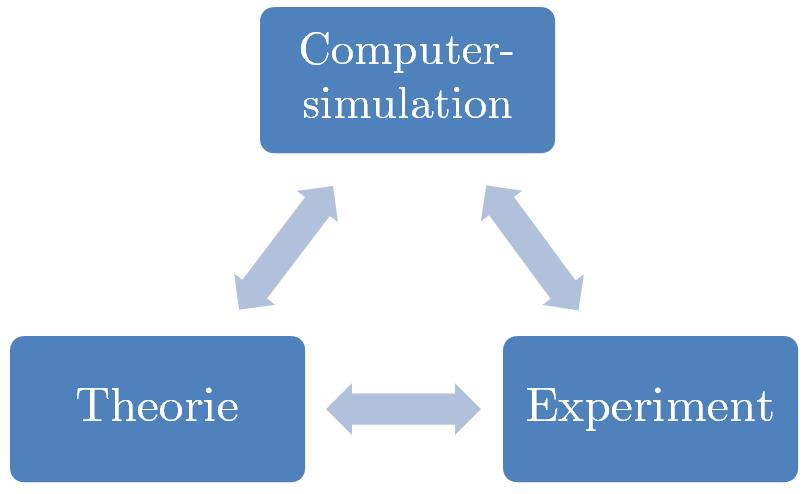
\includegraphics[width=0.45\textwidth]{Null_DrittesStandbein.jpg}
	%\caption{}
	\label{Null_DrittesStandbein}
\end{figure}
\begin{itemize}
\item Vorteile:

\begin{itemize}
\item löst Probleme für die es keine analytische Lösung gibt
\item schafft Raum für Modelle, zu denen es keine analytischen Verfahren gibt
\item kann physikalische Größen berechnen, die nicht messbar sind 
\item immer leistungsfähiger
\item immer billiger
\end{itemize}


\item Vorgehensweise:

\begin{itemize}
\item Modellierung: realistisch $\longleftrightarrow$ einfach
\item Programmierung / Test
\item Erzeugen von Daten / Optimierung
\item Analyse / Interpretation
\end{itemize}

\subsection{Hardware}
Diese Vorlesung beschäftigt sich nicht mit Hardware an sich, aber wir müssen abschätzen, ob ein Problem nummerisch lösbar ist! 

\underline{Beispiel:} Wie weit kann ein Rechner zählen?
\begin{align*}
S(N)= \sum_{i=1}^N x_i \; \mbox{  beispielsweise mit: } x_i = 1
\end{align*}
\end{itemize}

\begin{enumerate}
\item \textbf{Rechenleistung:} 
typisch 10 GFLOP/S ('\textbf{G}igia \textbf{F}loating \textbf{P}oint \textbf{O}perations \textbf{P}er \textbf{S}econd', Gleitkommazahlen Operationen) \\
\underline{Zum Beispiel Additionen:} \\
Bei $N=10^{10} $ pro Sekunde \\
$\Rightarrow$  Für die Zahl der Atome  ($N = 10^{23}$) dann $10^{13} s \approx 3 \cdot 10^5 a$

\item \textbf{S}
\end{enumerate}

\section{Monte Carlo Verfahren}
\subsection{TIDIIII}
\subsection{ Monte Carlo Integration}
Betrachten Integral 
\begin{align}
I= \int_a^b f(x) \; dx
\end{align}
Konventionelle nummerische Methode: Zerlegung in Intervalle $\Delta x$:

\begin{align}
I_n= \sum_{\nu =1}^n f(x_\nu) \; , \mbox{ Rechteckregel, für } n \to \infty
\end{align}
$\Rightarrow I_N \to I$ (falls integrierbar).

Besser ist die Trapezregel, Simpson, Konvergenz verschieden

Verallgemeinerung auf höhere Dimensionen:

d-dimensional, $n$ Stützstellen pro Achse $\Rightarrow n^d$ Hypercubi der Göße $(\Delta x)^d$ und damit $\Rightarrow n^d$ Terme summieren
Beispiel: Phasenraumintegral: 3TL, Freiheitsgrade $\vec{r}, \vec{p}$

\begin{align}
\int d^3 \vec{r}_1 d^3 \vec{r}_2 d^3 \vec{r}_3 d^3 \vec{p}_1 d^3 \vec{p}_2 d^3 \vec{p}_3 .... 
\end{align} %TODO bild
ist 118 dimensional mit $n=100, d=18 \Rightarrow n^d=100^18=10^36$. Bei $10^10$FLOPS
$\Rightarrow$ Summation dauert $10^{36 } / 10^{10}= 10^{26}s$ (Vergleich: alter des Universums ist $10^{19}s$.)
Wir brauchen also andere Methoden der Statistik:

Betrachten wieder 
\begin{align}
I= \int_a^b f(x) \; dx
\end{align}
mit $x_1,....x_N$ seine $N$ gleichverteilte Zufallszahlen über $[a,b]$ %TODO bild

$N_\mu$ sei Anzahl der $x_i$ im $\nu$ten Teilintervall dann gilt
\begin{align}
n \cdot \Delta x =& b-a \; \\
\Rightarrow \frac{\bar{N}_\nu}{N}=& \frac{1}{n}= \frac{\Delta x}{b-a} \\
\Rightarrow I= & \int_a^b f(x) \; dx \approx \sum_{\nu =1}^n (b-a)  \frac{\bar{N}_\nu}{N} f(x_0) \\
=& \frac{b-a}{N} \sum_{\nu =1}^n \underbrace{\bar{N}_\nu f(x_0)}_\text{( * )}
\end{align}
mit *$ \approx \sum_{x_j \leftarrow [ ]_\nu} \; f(x_j)$.
Dies gilt auch in höheren Dimensionen:
\begin{align}
I \approx \frac{v_\nu}{N} \sum_{i=1}^N f(\vec{x}_i)
\end{align}
Mittelwert der Funktionswerte an zufälligen Stützstellen $\vec{x}_i$.
\textbf{Fehler:} $\{ x_1, x_2,..., x_N\}$ sei spezielle Folge von Zufallszahlen mit $I_1$ als Resultat. Andere Folge erzeugt $I_2,...$ 
$\Rightarrow$ Es gibt eine Wahrscheinlichkeitsverteilung $P(I)$ %TODO image
betrachte deswegen unendliche (exaktes Resultat, aber wie groß ist dann die Schankung) viele Ketten von Zufallszahlen der Länge $N$: $\Rightarrow P(I) dI$ wäre dann die Wahrscheinlichkeit, dass $I$ im Intervall $I$ liegt.
\begin{align}
\langle I \rangle =& \int dI \; P(I) \; I \; \mbox{ mit } I= \frac{1}{N} \sum_{i=1}^N f(x_i)= I(x_1,x_2,...,x_N) \\
=& \int dx_1,...,dx_N \; \rho(x_1) ... \rho(x_N) \; \frac{1}{N} \sum_{i=1}^N f(x_i) \\
=& \int dx \; f(x) ,
\end{align}
unendlich viele Folgen von UZ gemittelt das exakte Ergebnis geben.

\textbf{Fehler:} 
\begin{align}
(I- \langle I \rangle)^2 \rangle =& \langle I^2 \rangle - \langle I \rangle ^2 \\
=& \langle \frac{1}{N^2} \left( \sum_{i=1}^N \; f(x_i) \right) ^2 \rangle - \langle \frac{1}{N} \sum_{i=1}^N \; f(x_i)\rangle^2 \\
=& \frac{1}{N^2} \sum_{i,j=1}^N \langle f(x_i) \; f(x_j) \rangle - \frac{1}{N^2} \sum_{i,j=1}^N \langle f(x_i) \rangle \; \langle f(x_j) \rangle \\
=& \frac{1}{N^2} \sum_{i=1}^N \langle f(x_i)^2 \rangle - \frac{1}{N^2} \sum_{i=1}^N \langle f(x_i) \rangle ^2 \; + O \mbox{ weil } \\
\langle f(x_i) \; f(x_j) \rangle = \langle f(x_i) \rangle \; \langle f(x_j) \rangle \; \mbox{ für } i \neq j
\end{align}
benutze
\begin{align}
\int dx_1 \; dx_2 \rho(x_1) \rho(x_2) f(x_1) f(x_2) \\
= \int dx_1 \rho(x_1)f(x_1)  \underbrace{\int dx_2 \rho(x_2)}_\text{=1}\cdot  \int dx_2 \rho(x_1)f(x_2) \cdot \underbrace{\int dx_1 \rho(x_1)}_\text{=1} \\
\Rightarrow \langle \Delta I \rangle ^2= \frac{1}{N} \left( \langle f(x)^2 \rangle - \langle f(x) \rangle^2 \right)
\end{align} 
Diskussion:
\begin{itemize}
\item[1)]
\begin{align}
\Delta I \propto \frac{1}{\sqrt{N}}
\end{align}
Zum Vergleich: Trapezregel. Fehler $\propto h^2 $, $N$ Rechenschritte: $h \propto N^{ \frac{-1}{d} }$ in $d$ Dimensionen. $\Rightarrow \Delta I \propto N^{\frac{-2}{d}} \Rightarrow$ für $d<4$ ist Monte Carlo 'besser'.

\item[2)] $I \to \langle I \rangle$ für $N \to \infty$. Ein $\infty$-lange Kette führt zum exakten Resultat (sebstmittelnd)

\item[3)] Verfahren gut, wenn $f$ konstant. %TODO bild
\item[4)]Fehler lässt sich bei der Integration berechnen.
\end{itemize}
Beispiel: Volumen einer D-Dimensionalen Einheitskugel. 

2D: %TODO bild
\begin{align}
f(x,y)=
\begin{cases}
1 & x^2+y^2 <1 \\
0 & \mbox{sonst}
\end{cases}
\end{align}
\begin{align}
I= \int_0 dx \; dy 1 = \int_{-1}^1 dx \int_{-1}^1 dy \; f(x,y) 
\approx \frac{4}{N} \sum_{i=0}^N f(x_i,y_i)
\end{align}
Zeige Programm: Volumen für hohe dimension verschwindet: Eindimensionale Betrachtung: Intervall geht exakt von $[-1,1]$, bei einem Kreis in $[-1,1] \times [-1,1]$ fallen schon die Ecken weg. Das Volumen auf den Einheitsradius ist nicht mehr ganz so groß. Bei drei Dimensionen fallen schon die 8 Ecken weg...daher nimmt das relatives Volumen ab für große Dimensionen.
Wie kann man das Verfahren verbessern?

\subsubsection{Verbesserung}:
\begin{align}
(\Delta I )^2 = \frac{1}{N} \underbrace{\left( \langle f^2(x) \rangle - \langle f(x)\rangle^2 \right)}_\text{Schwankungsbreite der Fkt}
\end{align}
Idee: Transformation, so dass der Integrand $\approx const$, dafür aber Zufallszahl nicht gleichverteilt.
\begin{align}
I= \frac{1}{N} \sum_{i=1}^N \frac{f(y_i)}{w(y_i)}
\end{align}
wobei $y_i$ eine Folge von ZZ mit Verteilung $w(y)$ mit $w(y)>0$, $\int w(y) \; dy=1$.
Beweis:
\begin{align}
\langle I\rangle = \langle \frac{1}{N} \sum_{i=1}^N \frac{f(y_i)}{w(y_i)} \rangle = \frac{1}{N} \sum_{i=1}^N \langle \frac{f(y_i)}{w(y_i)} \rangle = \frac{1}{N} \sum_{i=1}^N \int dy_i \; w(y_i)  \frac{f(y_i)}{w(y_i)} 
= \int dx \; f(x)
\end{align}
Fehler: \begin{align}
I=\frac{1}{\sqrt{N}}
 \sqrt{\langle \left(\frac{f}{w}\right)^2 \rangle - \langle \frac{f}{w} \rangle ^2}
 \end{align}
 $\Rightarrow$ für kleine Felder: $w$ so wählen, dass $\frac{f}{w} \approx const.$ Man muss allerdings $w$ integrieren können. %TODO grafik
 
 $\Rightarrow$ Mann nennt dieses Verfahren:\textbf{Importance sampling}, weil 'wichtige' Werte von $f(x)$ in der ursprünglichen Funktion häufiger vorkommen, gegensätzlich zu \textbf{simple sampling} $\to$ die Wurzel N im Fehler ist geblieben. Leider konnten wir die Konvergenz dadurch nicht verstärken. Neues Problem hierbei ist jetzt: 
 
 \subsection{Zufallszahlen einer vorgegebenen Verteilung}
 Problem: %TODO grafik
 Zufallszahlen $x_i$ aus Intervall berechnen mit einer Verteilung $\rho(x)$ mit $\rho(x)>0, \int_0^1 dy \rho(x)=1$.
 \begin{itemize}
 \item[a)] Rejection-Method nach von Neumann \\
 %TODO grafik
 betrachte Paar von Zufallszahlen, $x_i \in [0,1], y_i \in [0,b]$ mit $b=Max[\rho(x)]$.
 
$\to$ wenn $y_i < \rho(x_i) \Rightarrow x_i$ wird akzeptiert mit $\xi_i=x_i$\\
 $\to$ wenn $y_i > \rho(x_i) \Rightarrow x_i$ wird nicht akzeptiert. \\
 
 $\Rightarrow$ Folge von Zufallszahlen $\xi_i$. Zahl der $\xi_i \in \Delta x$ ist proportional zur Fläche $\rho(x) \Delta x$ und damit proportional zu $\rho(x)$.
 
 \textbf{Problem:} viele Züge notwendig, wenn selten akzeptiert wird. 
 
 \textit{Schlecht wäre zum Beispiel:} die Betrags-Exponentialfunktion
 %TODO image
 
\textit{Gut wäre dafür aber:}
Vektoren mit (oder auf) Einheitskreis
%TODO

\item[b)] Transformationsmethode \\
betrachte monotone Funktion. Dabei seien wieder $x_i$ gleichverteilte Zufallsvariablen aus $x_i \in [0,1]$ und $y_i = f(x_i)$. Wie sind die verteilt? (Dafür muss man die Wahrscheinlichkeiten umrechnen. In ein $\Delta x$ fallen irgendwelche Zufallsvariablen rein und werden auf $\Delta y$ abgebildet, das ja kleiner sein kann. Die dichte in $\Delta y$ sowie $\Delta x$ kann also verschieden sein.) %TODO siege image

$N$ Zufallszahlen, $\Rightarrow$ $N \cdot \Delta x$ fallen in das Intervall $\Delta x$. Die entsprechenden abgebildeten Zufallszahlen $y_i=f(x_i)$ fallen in $\Delta y$.

$\Rightarrow$ Änderung der Punktdichte $\rho(y)\Delta y = \Delta x$. Im limes $\Delta x \to 0$ mit 
\begin{align*}
\rho(y)=\frac{dx}{dy}
\end{align*}
soll vorgegeben werden
\begin{align}
\Rightarrow & \int_0^x dx' = \int \rho(y) dy \; \Rightarrow \; x(y) = \int \rho(y) dy = f^{-1}(y) \\
\Aboxed{\Rightarrow & f(x)= \left( \int \rho(y) \; dy \right)^{-1} }\\
\Rightarrow & f(x_i)=y_i \mbox{ sind gesuchte ZZ}
\end{align} %TODO frameon the last formula
also: $\rho(y)$ gegebene Verteilung muss man 1) Integrieren 2) Invertieren
 
 Beispiel: \begin{align}
  \rho(y)=
 \begin{cases}
e^{-y} & \text{für } y \geq 0 \\
0 & \text{für } y < 0.
 \end{cases}
 \end{align}
 
 \begin{enumerate}
 \item \begin{align*}
 \int_0^y dy' \rho(y') = 1_ e^{-y} =x(y)
 \end{align*}
 \item Umkehrfunktion:
  \begin{align*}
 y= - ln(1-x) = f(x)
 \end{align*}
 $\Rightarrow$ ziehe gleichverteilte Zufallszahl $x_i \in [0,1)$ (nicht die 1 selber!) \\
 $\Rightarrow y_i = -ln(1-x_i)$ sin exponentiell verteilte Zufallszahlen $\in [0,\infty]$.
 \end{enumerate}
 Nachteil: 
(Der Computer ist nicht so schnell beim logarithmieren...deswegen ist die rejection Methode diesbezüglich interessanter.) 
Man muss aber vor allem die gewünschte Verteilung $\rho(y)$ erst integrieren und dann invertieren können. Dies geht beispielsweise nicht bei:

\item[c)] Gauß-Verteilung
\begin{align*}
\rho(x)= \frac{1}{\sqrt{2 \pi} \sigma} e^{-\frac{x^2}{2 \sigma^2}}
\end{align*}
denn sie ist nicht analytisch bestimmt integrierbar. Dafür gibt es einen Trick:

Trick: betrachte eine zweidimensionale Verteilung:
\begin{align*}
p(x_1,x_2)=\frac{1}{	2 \pi \sigma^2} e^{- \frac{x_1^2 + x_2^2}{2 \sigma^2}}
\end{align*}
Zahl der Punkte im Intervall $dx_1, dx_2$ ist:
\begin{align*}
\frac{1}{	2 \pi \sigma^2} e^{- \frac{x_1^2 + x_2^2}{2 \sigma^2}} dx_1 dx_2= & \frac{1}{	2 \pi \sigma^2} e^{- \frac{r^2}{2 \sigma^2}} \;r \; dr  d\phi \; \mbox{  subst: } u = \frac{r^2}{2 \sigma^2}\\
= & \frac{1}{2 \pi} e^{-u} du \; d\phi \\
\end{align*}
mit
\begin{align*}
x_1=  r cos(\phi) = \sigma \sqrt{2 u} cos(\phi) \\
x_2=  r sint(\phi)= \sigma \sqrt{2 u} sin(\phi)
\end{align*}
$\Rightarrow$ ziehe Zufallszahl $\phi_i$ aus $[0,2\pi]$, $y_i$ ist exp-verteilt aus $[0, \infty]$.

rechne $x_1,x_2$....

praktisch: \begin{align}
\Aboxed{x_{2i}= \sigma \sqrt{-2 ln(1-y_{2i})} \; cos(2\pi \; y_{2i-1}) } \; \mbox{ mit } y_i\mbox{ ZZ} \in [0, 1) \mbox{ gleichverteilt}
\end{align}
Beispiel: Wir nehmen das Integral
\begin{align*}
\int_0^{2\pi} x e^x \; dx \underbrace{=}_\text{analytisch} e^{2\pi} (2\pi -1) +1
\end{align*} 
Importance: \begin{align*}
\rho(y)=& \frac{e^y}{e^{2\pi} -1} \mbox{ (normiert) } \Rightarrow f(x)= ln(\underbrace{(e^{2\pi}-1)}_\text{Norm.-Konst} x+1) \\
\Rightarrow & I = \frac{1}{N} \sum_{i=1}^N y_i (e^{2\pi}-1)
\end{align*}
\end{itemize}
 
 %TODO Review:
 Importance sampling: \begin{equation}
 i= \frac{1}{N} \sum_{i=1}^N \frac{f(y_i)}{w(y_i)} \mbox{ mit } y_i: \mbox{ ZZ normalverteilt }
 \end{equation}
 
 Beispiel: \begin{align}
 \int_0^{2\pi} x \; e^x \; dx = e^{2\pi} (2\pi -1) -1\\
 w(y)= \frac{e^y}{e^{2\pi}-1} \\
 y= ln\left( (e^{2\pi} -1)x+1\right) \mbox{ mit } x \in [ 0,1] \\ \Rightarrow I= \frac{1}{N}\sum_{i=1}^N y_i (e^{2\pi}-1)
 \end{align}
 %TODO Review END
 
 \subsection{Ising Modell}
(Zweizustandsmodell: minimales Modell für ein reales system, jeder einzelne Freiheitsgrad hat nur zwei zustände, ist aber das erste Modell das einen Phasenübergang zeigt. Es ist im 2D Fall aber exakt lösbar und daher gut für uns.)
\begin{itemize}
\item[-]Findet zahlreiche Anwendungen
\item[-]einfach
\item[-]exakte Lösungen im 1D,2D Fall

 hier: Modell für Ferromagneten %TODO Gitterbild: zweizustandsmodell: dargestellt: möglicher zustand
 (Die Wechselwirkung ist im einfachsten Fall nur mit den nächsten Nachbart, idee: überlapp der wellenfunktion ist begrenzt exponentiell...)
\item[-] Gitter aus Spins, im einfachsten Fall $S= \pm 1$, sodass beispielsweise $S_i$ nur index $i= \{x,-\}$ hat.
\item[-]Hamilton-Funktion $H= - \sum_{i=1}^N B \; S_i$ (Spin hier kein Drehimpuls sondern Spin, das minus kommt vom Drehimpuls des \textit{Elektrons}. Es ist ein phänomenologisches klassisches Modell, also nicht wirklich ein quantenmechanisches Spin-$1/2$-Modell sonder im klassischen Limes (Limes Heisenbergmodell und gleichzeitig anisotropie gegen unendlich)) 
 \item[-]Hinzüglich einer Wechselwirkung: Austauschenergie J zwischen Spinpaaren. Am stärksten zwischen nächsten Nachbarn $ H= -J \sum_{i,j=1\; und \; i,j NN}^N S_i S_j - B \sum_{i=1}^N S_i$ ($B$ gibt vor, welche ausrichtung energetisch günstiger ist. Beispiel: $\uparrow \uparrow, B: \Uparrow$)
  \begin{itemize}
  \item $J>0: \; \uparrow \uparrow $ günstig $\rightarrow$ Ferromagneten
  \item $J<0: \; \uparrow \downarrow$ günstig $\rightarrow$ eventuell Antiferromagneten ($\uparrow \downarrow \; , \; \downarrow \uparrow$)
  \end{itemize}

\begin{enumerate}
\item Grundzustand (Kette): $E_0= -J(N-1)-BN $. $\uparrow \uparrow \uparrow \uparrow \uparrow \uparrow$
\item Endliche Temperatur $T$: angeregte Zustände, z.B. $\uparrow \uparrow \uparrow \downarrow \uparrow$ \textit{(erster angeregter Zustand)}
\end{enumerate}

\underline{Thermische Mittelwerte:} Observable $\Omega: \langle \Omega \rangle= \sum_{ \{\bar{S} \} \\ 2^N }  p(\bar{S}) \Omega(\bar{S})$ mit $\bar{S}:$ Zustand, $\Omega(\bar{S})$: Observable, $p(\bar{S}):$ Wahrscheinlichkeit von $\bar{S}$. %TODO richtig plaziert?

\item[-] kanonische Gesamtheit 
\begin{align}
p_{\bar{S}}=p(H(\bar{S})= \frac{e^{- \beta H(\bar{S})}}{\sum_{\{ \bar{S} \} } e^{-\beta H(\bar{S})}} \; , \; \beta = \frac{1}{k_BT}
\end{align}
mit \textit{Zustandssumme} 
\begin{align}
Z= \sum_{ \{\bar{S}\} } e^{- \beta H(\bar{S})} \mbox{ und } \langle \Omega \rangle = \frac{1}{Z}  \sum_{ \{\bar{S}\} } \Omega(\bar{S}) e^{- \beta H(\bar{S})}
\end{align} (fürs kanonische Ensemble bestimmbar in obiger Form)


\end{itemize}
Beispiel ($N=2$): 
Magnetisierung $\langle M \rangle = \frac{1}{Z} \sum M e^{- \beta H(S_1,S_2)}$ mit $M= \frac{1}{N} \sum_{i=1}^N S_i$.
\begin{align*}
2^N \mbox{ Zustände } \uparrow \uparrow \; \downarrow \uparrow \; \uparrow \downarrow \; \downarrow \downarrow
\end{align*}
\begin{align*}
Z= e^{-\beta (-J -2B)} + 2 e^{-\beta J} + e^{- \beta (-J +2B)} \\
\langle M \rangle = \frac{1}{2} \frac{2 e^{-\beta (-J - 2B)} - 2 e^{-\beta (-J + 2B)}}{Z}
\end{align*} %TODO image

\subsection{Monte Carlo Simulation}
(Wir rechnen im kanonischen Ensemble die Zustandssumme aus.)
\begin{align}
\langle M \rangle =& \frac{\sum^{2^N}_{\bar{S}} M(\bar{S}) e^{-\beta H(\bar{S})}}{\sum^{2^N}_{\bar{S}} e^{-\beta H(\bar{S})}}  \\ \underbrace{\approx}_\text{simple sampling} &
\frac{\sum^{k}_{\bar{S}} M(\bar{S}) e^{-\beta H(\bar{S})}}{\sum^{k}_{\bar{S}} e^{-\beta H(\bar{S})}} \mbox{ nicht alle } 2^N \mbox{Zustände sondern } k \\
\underbrace{\approx}_\text{importance sampling} & 
\frac{\sum^{k}_{\bar{S}} M(\bar{S}) e^{-\beta H(\bar{S})} \frac{1}{w(\bar{S})}}{\sum^{k}_{\bar{S}} e^{-\beta H(\bar{S})} \frac{1}{w(\bar{S})}}
\end{align}

wähle $w(\bar{S})= e^{-\beta H(\bar{S})} $ und dann folgt

\begin{align}
\Aboxed{ \langle M \rangle = \frac{1}{K} \sum_{ [\bar{S}]}^{(k)} M(\bar{S})}
\end{align}
$\Rightarrow$ Problem: wir brauchen Zustände $\bar{S}$ mit Wahrscheinlichkeit $w(\bar{S})\propto e^{-\beta H(\bar{S})}$ ($\Rightarrow$Problematisch). Wie bekommt man jetzt Konfigurationen mit einer bestimmten Wahrscheinlichkeitsverteilung? 
Lösung: Metropolis-Algorithmus.

Beginne einen Markov-Prozess (Kette) , (meint dass der nächste Zustand hängt nur von seinem Vorgänger ab, d.h. ein Zustand wird vom Vorgängerzustand erzeugt:) $\bar{S}_0 \rightarrow \bar{S}_1 \rightarrow \bar{S}_2$
beispielsweise $\uparrow \uparrow \uparrow \; \rightarrow \; \uparrow \downarrow \uparrow \; \rightarrow \; \uparrow \downarrow \downarrow$
\begin{enumerate}
\item $\bar{S}_n $ sei ein Zustand
\item \label{Punkt2} erzeuge Versuchszustand (trial state) $\bar{S}_r$ durch \textit{geeignete} Veränderung.
\item berechne: 
\begin{align}
r= \frac{w(\bar{S}_r)}{w(\bar{S}_n)} = e^{-\beta (H(S_r)-H(S_n))}
\end{align}
\item Fallunterscheidung: \\ 
$r>1$: akzeptieren, $\bar{S}_{n+1} = \bar{S}_r$\\
$r \leq 1:$ akzeptieren mit Wahrscheinlichkeit $r$
\item  $\rightarrow$ \ref{Punkt2}.
\end{enumerate}
Implementierung: am Beispiel einer Spinkette $\uparrow \uparrow \uparrow \uparrow \uparrow \uparrow$ (der letzte wechselwirkt mit dem ersten wieder...periodische Randbedingungen also)
\begin{enumerate}
\item Array von Spins $spins[N]$: $ +1|+1|+1|+1|+1|+1|$
\item \label{wiederPunkt2} Versuchsschritt: misst 'single spin flip' $S_i \rightarrow - S_i$: $ +1|-1|+1|+1|+1|+1|$
\item $\Delta H= H(\bar{S}_r)  - H(\bar{S}_n) = 2 J (S_i S_{i-1} + S_i S_{i+1}) + 2BS_i \; \; \Rightarrow r= e^{-\Delta H / k_BT}$
\item \texttt{if (rand()/Randmax $<$r)} $S_r \rightarrow -S_i$
\item $\rightarrow$ \ref{wiederPunkt2}.
\end{enumerate}

\begin{itemize}
\item Wenn alle Spins einmal abgefragt wurden: $1MCS$ (MonteCarloSchritte)
\item Mittelung über viele MCS

\item Zu Beginn der Simulationen ist der Markov Prozess nicht im Gleichgewicht (hängen vom Anfangszustand ab) $\Rightarrow$  die ersten $k$ MCS sollten nicht zur Mittlung herangezogen werden: \begin{align}
\langle M \rangle = \frac{1}{(K-k)} \sum_{i=k}^K M_i \mbox{ mit } M_i = \frac{1}{N} \sum_{j=1}^N S_j
\end{align}
Beweis: Metropolis erzeugt Konfiguration $\bar{S}$ mit einer Wahrscheinlichkeitsverteilung von $w(\bar{S}) \propto e^{-\beta H(\bar{S})}$ (Wie betrachtet man denn nun statistische nicht gleichgewichtsprozesse so wie diesen Markov Prozess?)
\item $w(\bar{S}):$ Wahrscheinlichkeit im Zustand $\bar{S}$ zu sein.
\item Markov $\bar{S} \rightarrow \bar{S'}$ mit $p(\bar{S}, \bar{S'}): $ Wahrscheinlichkeit, im Prozess von $\bar{S}$ nach $\bar{S'}$ zu wechseln

Aufgabe: $p$ bestimmen, sodass $w(\bar{S})$ herauskommt
\end{itemize} %TODO bild mit strichen
\begin{align*}
\Delta w(\bar{S}) =& 
- \sum_{\bar{S'}} w(\bar{S}) p(\bar{S} \rightarrow \bar{S'}) \mbox{ (raus) } \\
 &+  \sum_{\bar{S'}} w(\bar{S'}) p(\bar{S'} \rightarrow \bar{S}) \mbox{ (rein) } \\ 
 \overset{!}{=}& 0
\end{align*}

%TODO ising modell: phasenübergang bei 2....irgendwas. Schwankungen in der reduzierten magnetisierung für werte kurz unter 2 kommen durch spezifische Wärmekapazität als schwankung der Energie und genauso die spezifische suszeptibilität als schwankung der Magnetisierung. Die zahl der Montecarlo schritte steigt bis man im gleichgewicht ankommt für steigende werte für T. Sie fällt für höhere werte detulich größer aus bis sie bei Null ankommt

Betrachte eine mögliche Lösung: jeder Summand $=0$. (\textbf{'detailed balance'}).
 \begin{align}
\Rightarrow   w(\bar{S}) p(\bar{S} \rightarrow \bar{S}')- w(\bar{S}') p(\bar{S}' \rightarrow \bar{S}) =0 \\
\Rightarrow  \frac{p(\bar{S} \rightarrow \bar{S}')}{p(\bar{S}' \rightarrow  \bar{S})} = \frac{w(\bar{S}')}{w(\bar{S})} = e^{-\beta(E(\bar{S}')- E(\bar{S})}
\end{align}
\begin{enumerate}
\item \underline{Lösung:}
 \begin{align}
p(\bar{S} \rightarrow \bar{S}')
\begin{cases}
e^{-\beta(E(\bar{S}')- E(\bar{S})} \text{ für } \Delta E > 0 \\
1 \text{ sonst}
\end{cases}
\end{align} 
\item \underline{Lösung:}
\begin{align*}
p(\bar{S} \rightarrow \bar{S}') = \frac{1}{1+ e^{\beta \Delta E}} \mbox{, weil } \\ 
\frac{p(\bar{S} \rightarrow \bar{S}')}{p(\bar{S}' \rightarrow \bar{S})} = \frac{1+e^{-\beta \Delta E} }{1+e^{\beta \Delta E}} = \frac{e^{-\beta \Delta E} (e^{\beta \Delta E}+1)}{1+e^{\beta \Delta E}}= e^{-\beta \Delta E}
\end{align*}
(\textbf{Heat-bath algorithm})
\end{enumerate}
\subsection{Master Gleichung und Monte Carlo Dynamik}
Zusammenhang mit irreversibler Dynamik.

betrachte System im nicht-Gleichgewicht, das equilibriert (irreversibel) %TODO image
\begin{itemize}
\item Stellen uns vor, wir haben $\infty$ viele Kopien des Systems
\item Berechne nun die zeitliche Änderung der Wahrscheinlichkeit $p_r(t)$ (Wahrscheinlichkeit, das System zur Zeit $t$ im Zustand $r$ zu finden)
\item betrachte quantenmechanisches System im Kontakt mit einem Wärmebad
\begin{align}
\bar{H}_{gesamt} = \underbrace{ \bar{H}}_\text{System} + \underbrace{\bar{H}'}_\text{Wärmebad} + \underbrace{ \bar{H}_i}_\text{Wechselwirkung}
\end{align}
\item System sei im Zustand $r$, $\bar{H} \Psi_r = E_r \Psi_r$ mit Wahrscheinlichkeit $p_r(t)$.

\underline{Master Gleichung}
\begin{align}
\frac{dp_r}{dt}= \sum_s p_s \underbrace{w_{sr}}_\text{} - p_r \underbrace{w_{rs}}_\text{Übergangsraten}
\end{align}
\item Anwendung im Wärmebad
\begin{align}
w_{rs}= & \sum_{r',s'} p_{r'}' w_g(rr' \rightarrow ss') = \frac{1}{Z'} \sum_{r',s'}  e^{-\beta E_{r'}'} w_g (rr' \rightarrow ss') \mbox{ Wärmebad ist kanonisch! } \\
w_{sr}= & \frac{1}{Z'} \sum_{r',s'}  e^{-\beta E_{s'}'} w_g (ss' \rightarrow rr')
\end{align}
\item Energieerhaltung: $E_{r'}' + E_r = E_{s'}' + E_s$ (*)
\item Symmetrie im Gesamtsystem $w_g (rr' \rightarrow ss') = w_g (ss' \rightarrow rr')$(*)
\end{itemize}
aus (*) einsetzen folgt
\begin{align}
w_{sr}&= \frac{1}{Z'} \sum_{r',s'} e^{\beta (E_{r'}' -E_{s'}') } e^{-\beta E_{r'}'  w_g (rr' \rightarrow ss')} = w_{rs} \; e^{-\beta (E_r - E_s)} \\
& \Rightarrow  \frac{w_{sr}}{w_{rs}}= e^{-\beta (E_r - E_s)}
\end{align}
\underline{also:} Irreversible Dynamik eines Systems in Kontakt mit einem Wärmebad wird beschrieben durch Master-Gleichung $ frac{dp_r}{dt}= \sum_s( p_s(t) w_{sr} - p_r(t) w_{rs}) $ mit $\frac{w_{sr}}{w_{rs}}= e^{-\beta (E_r-E_s)}$. Diese Dynamik wird durch Metropolis Algorithmus (oder Heat Bath Algorithmus) simuliert.

\underline{Beachte:} \begin{itemize}
\item $w_{sr}$ liegen nicht absolut fest. Mit $w_{sr}, w_{rs}$ ist auch $\gamma (t) w_{sr}, \gamma(t) w_{rs}$ Lösung \\  $\Rightarrow$ Zeitskala ist nicht absolut festgelegt!
\item $w_{sr}$ ist nicht mikroskopisch bekannt (im Raum nicht festgelegt)
\item Die Master Gleichung beschreibt \textit{ausschließlich} irreversible Dynamiken!
\item speziell für Ising Modell heißt diese Dynamik Glauber-Dynamik.


\end{itemize}
Beispiel: Glauber Dynamik für 2 Spins:  $H=-J S_1 S_2$ mit $S_{1,2} = \pm 1$
$2^2 =4$ Zustände: $ \uparrow_+ \uparrow_+ \; \; \uparrow_+ \downarrow_- \; \; \downarrow_- \uparrow_+ \; \; \downarrow_- \downarrow_-$

 \begin{align*}
 \frac{dp_{++}}{dt} = \sum_s p_s w_{sr} - p_r w_{rs}
 \end{align*}
 (Energie $++$ und $--$ sind genau gleich, da ja kein externes Feld angelegt ist. Nur interessant ist also der Übergang von $++, --$ zu $+-,-+$) $\Rightarrow$ Annahme: Single spin flip und 'Metropolis' mit \begin{align*}
 w=
 \begin{cases}
 1 & \Delta E <0 \\
 e^{- \frac{\Delta E}{kT}} & \Delta E>0
 \end{cases}
 \end{align*}
 Es gibt 
 \begin{itemize}
 \item  $w_{++ \rightarrow --}= w_{+- \rightarrow -+}$ etc...
 \item $w_{+- \rightarrow ++}= w_{-+ \rightarrow ++}=1$ etc...
 \item $w_{-- \rightarrow -+}= w_{-- \rightarrow +-}= w= e^{-\frac{2J}{k_BT}}$ etc... 
 \end{itemize}
 
  \begin{align*}
 \frac{dp_{++}}{dt} =& \sum_s p_s w_{s \rightarrow ++} - p_{++} w_{++ \rightarrow s} \\
 =& p_{+-} w_{+- \rightarrow ++} - p_{++} w_{++ \rightarrow +-} +
 p_{-+} w_{-+ \rightarrow ++} - p_{++} w_{++ \rightarrow -+} =
 p_{+-} + p_{-+} - 2 p_{++} w \\
 \frac{dp_{--}}{dt}= & p_{+-} + p_{-+} - 2p_{--}w \\
  \frac{dp_{+-}}{dt}= & p_{++}w + p_{--} w- 2p_{+-} \\
   \frac{dp_{-+}}{dt}= & p_{++}w + p_{--}w -2p_{-+}
 \end{align*}
$\Rightarrow$ homogenes, lineares Gleichungssystem
$\Rightarrow$ Lösung für $\lambda$ mit 
\begin{align*}
\begin{vmatrix}
-2w+\lambda & 0 & 1 & 1 \\
0 & -2w +\lambda & 1 & 1 \\
w & w & -2w + \lambda & 0 \\
w & w & 0 & -2+\lambda 
\end{vmatrix} \\
\end{align*}
$\Rightarrow \lambda_1=0, \lambda_2=2, \lambda_3=2w+2, \lambda_4=2w$ \\
Wichtig: Kleinstes $\lambda >0$ definiert die Relaxationszeit
$\Rightarrow$ für lange Zeiten: $p_s(t) \approx a_s + b_s e^{-\lambda_4 t} \approx a_s + b_s e^{-\frac{t}{\tau}}$ mit $\tau= \frac{1}{20}= \frac{e^{2J/k_BT}}{2}$ \\
\underline{Magnetisierung:} $M(t)= \sum_s p_s(t) M_s = 2(p_{++}(t) + p_{--}(t) \approx M_0 e^{-\frac{t}{\tau}} + const$, wobei $const=0$. (Formel gilt für $t\to \infty$) \\
\underline{Diskussion:} %TODO image
\begin{itemize}
\item $\tau$ hängt vom 'Algorithmus' ab
\item $p(t)$ hängen von Dynamik ab (single spin flip oder nicht)
\end{itemize}
\subsection{Phasenübergange und Skalentheorie}
\begin{itemize}
\item[•] ideale Gase haben keine Wechselwirkung
\item[•] erst die Wechselwirkung zwischen Teilchen erklärt aber das Entstehen von Ordnung
\item[•] Ordnung entsteht häufig spontan durch PÜ, bei dem eine Symmetrie gebrochen wird.
\item[•]lösbares Modell: Ising-Modell: %TODO image
\end{itemize}
Ordungsparameter; $ lim_{B \to 0} lim_{N \to \infty} M(B)$.\\
Analytisch: 2D, Quadratgitter: \begin{align}
J= - \sum_{i,j} \frac{J}{2}\sigma_i \sigma_j \; , \; \sigma_i=\pm 1
\end{align}
Onsager: \underline{innere Energie:}
\begin{align}
\frac{U}{N}= &- J \; coth( \frac{2J}{k_BT}) \left[ 1 + \frac{2}{\pi} \left( 2 \; tanh^2 \left( \frac{2J}{k_BT} \right) - 1 \right) K_1(\kappa ) \right] \; \mbox{ mit} \\
\kappa=& \frac{2 \; sinh \left( \frac{2J}{k_BT} \right)}{cosh^2 \left( \frac{2J}{k_BT} \right) } \; , \; K_1(\kappa)= \int_0^\frac{\pi}{2} \frac{1}{\sqrt{1- \kappa^2 \; sinh^2(\Phi)}} d\Phi
\end{align}
U ist nicht analytisch bei einer Temperatur $T_c$ mit $sinh(\frac{2J}{k_BT_c} ) = 1 \Rightarrow cosh(\frac{2J}{k_BT_c})= \sqrt{2} \Rightarrow 2 tanh^2( \frac{2J}{k_B T_c}) =1$ mit $k_B T_c = 2.269 J$. %TODO bild
\begin{itemize}
\item[•] spezifische Wärme $c(T \to T_c) \propto - ln \left(\vert 1- \frac{T}{T_c}\vert \right)$
\item[•]Magnetisierung 
\begin{align}
m=
\begin{cases}
0 & T>T_c \\
\sqrt[4]{1+x^2} \sqrt[8]{1-6x^2 +x^4} & T<T_c
\end{cases}
\end{align}
\item[•]PÜ (Phasenübergang) $2.$Ordnung, Ordnungsparameter stetig, kritische Exponenten
\end{itemize}
kritische Exponenten beschreiben Verhalten in der Nähe des kritischen Punktes $(\epsilon = \frac{T - T_c}{T_c} , B) = (0,0)$ \\
spezifische Wärme: $c \propto \epsilon^{-\alpha}$\\
Suszeptibilität: $\chi \propto \epsilon^{-\gamma}$\\
Korrelationslänge: $\xi \propto \epsilon^{-\nu}$\\ 
Magnetisierung (OP) \begin{align}
m= \begin{cases}
M \propto \epsilon^{-\beta} & T<T_c \\
M \propto \vert B \vert ^\frac{1}{\delta} & T=T_c
\end{cases}
\end{align}
genauer: \begin{align*}
A(\epsilon)= 
\underbrace{ A_0 + A_1 \epsilon + A_2 \epsilon +...}_\text{analytisch} 
+ \underbrace{ A_3 \epsilon^{0.8}}_{\substack{ \text{führend} \\ \text{ nichtanalytisch} \\ \text{ (kritisch)} }}
+ \underbrace{ A_4 \epsilon^{1.7}}_\text{Korrekturen}
\end{align*}
\underline{wichtig:} Universalität \\
\underline{Skalenhypothese:} Freie Energie ist eine verallgemeinerte, homogene Funktion: \begin{align}
G(a^{x_1} B, a^{x_2} \epsilon)= a \; G(B, \epsilon)
\end{align} 
für führenden nicht-analytischen Anteil. \\
'normal' wäre: $U( \lambda S, \lambda V, \lambda N) = \lambda U(S,V,N))$ \\
Beispiel: $f(x) = x^{0,5} \Rightarrow f(bx) = (bx)^{0,5} = b^{0,5} x^{0,5}$ \\ \begin{align*}
b=a^2 \;  \Aboxed{ f(a^2 x)=  a x^{0,5} = a f(x)}
\end{align*}
'normal' f analytisch $\Rightarrow f(x)= f(0) + f'(0)x + .... \Rightarrow \Delta f(x) = f(x) - f(0) = f'(0)x+...$
\begin{align}
\Rightarrow \Aboxed{ \Delta f(ax) = f'(0) ax= a \Delta f(x)}
\end{align}
\underline{Folgerungen:} setze $ a= \vert \epsilon \vert ^{-1/x^2}$
\begin{align}
\Rightarrow G\left(\vert \epsilon \vert ^{-\frac{x_1}{x_2}} B, \underbrace{ \frac{\epsilon}{\vert \epsilon \vert}}_{\pm 1} \right) = \vert \epsilon \vert^\frac{-1}{x^2} G(B, \epsilon)
\end{align}
\underline{Definition:} Skalenfunktion: \begin{align}
f^\pm \left( \frac{B}{\vert \epsilon \vert ^\frac{x_1}{x_2}} \right) = G \left( \epsilon^\frac{-x_1}{x_2} B, \pm 1 \right)
\end{align} 
\underline{Skalenhypothese:}
\begin{align}
G(B,\epsilon) = \vert \epsilon \vert ^\frac{1}{x_2} \; f^\pm \left( \frac{B}{\vert \epsilon \vert ^\frac{x_1}{x_2}} \right) \\
G(B,\epsilon) = \vert B \vert ^\frac{1}{x_1} \; g \left( \frac{\epsilon}{\vert B \vert ^\frac{x_2}{x_1}} \right)
\end{align}
\begin{itemize}
\item[•]Eigenschaften der Skalarfunktionen $g,f$: G soll am kritischen Punkt endlich bleiben $\Rightarrow f^\pm (0)$ und $g(0)$ bleiben endlich (und ihre Ableitungen) $\Rightarrow \alpha, \beta, \gamma, \delta$ lassen sich durch $x_1, x_2$ ausdrücken: \\
\underline{spezifische Wärme:} \begin{align}
G(0, \epsilon)= \vert \epsilon \vert
^\frac{1}{x_2} f^\pm (0) \; , \; B=0 \\
\Rightarrow c \propto \frac{\partial^2 G}{\partial \epsilon^2} \propto \vert \epsilon \vert ^{\frac{1}{x_2}-2}= \vert \epsilon \vert ^{-\alpha} \; , \; \Rightarrow \alpha = 2- \frac{1}{x_2} 
\end{align}
\underline{spontane Magnetisierung:} 
\begin{align}
M(0,\epsilon) \propto \frac{\partial G(B, \epsilon)}{\partial B} \vert \epsilon \vert ^\frac{1}{x_2} f^\pm \left(\frac{B}{\vert \epsilon \vert ^\frac{x_1}{x_2}} \right) \propto \vert \epsilon \vert ^\frac{1}{x_2} \frac{1}{\vert \epsilon \vert ^\frac{x_1}{x_2}} \propto \vert \epsilon \vert ^\beta \Rightarrow \beta = \frac{1-x_1}{x_2}
\end{align}
\underline{Suszeptibilität:}
\begin{align}
\xi = \frac{\partial M}{\partial B} \Bigg\vert_{B \to o}
 \propto \vert \epsilon \vert ^\frac{1}{x_2} \frac{1}{\vert \epsilon \vert ^\frac{2 x_1}{x_2}} \Rightarrow \gamma = \frac{2x_1 -1}{x_2}
\end{align}
\underline{Magnetisierung für $\epsilon =0$:}
\begin{align}
M(B,\epsilon) = - \frac{\partial G}{\partial B} = - \frac{\partial}{\partial B} \left[ \vert B \vert ^\frac{1}{x_1} g\left( \frac{\epsilon}{\vert B \vert ^\frac{x_2}{x_1}} \right) \right] \\
= - B^{\frac{1}{x_1}-1} g\left( \frac{\epsilon}{B^\frac{x_2}{x_1}}\right) - \vert B \vert ^\frac{1}{x_1} \frac{x_2}{x_1} \frac{\epsilon}{\vert B \vert ^{\frac{x_2}{x_1}+1} } g'\left( \frac{\epsilon}{\vert B \vert ^\frac{x_2}{x_1} }\right) \\
= - B^{\frac{1}{x_1}-1} \left[ 
g\left( \frac{\epsilon}{B^\frac{x_2}{x_1}}\right) 
- \frac{x_2}{x_1} \frac{\epsilon}{\vert B \vert ^{\frac{x_2}{x_1}} } g'\left( \frac{\epsilon}{\vert B \vert ^\frac{x_2}{x_1} }\right) \right] \\
\Rightarrow \Aboxed{M(B,\epsilon)= B^\frac{1}{\delta} \text{\~{g}} \left( \frac{\epsilon}{B^\frac{1}{\beta \delta}} \right)  }\\
\frac{M(B,\epsilon)}{\underbrace{B^\frac{1}{\delta}}_\text{Grösse hängt von einem Feld ab}}=  \text{\~{g}} \left( \frac{\epsilon}{\underbrace{ B^\frac{1}{\beta \delta}}_{ \substack{ \text{hängt von} \\ \text{zwei Feldern} \\ \text{ ab}}}} \right) 
\end{align} %TODO formel schöner
\underline{vorher:} $M = M(B,\epsilon)$ \\ %TODO image
\underline{Crossover-Verhalten} \\
Skalarverhalten: \begin{align}
G(B,\epsilon)=& \vert \epsilon \vert ^\frac{1}{x_2} f^\pm \left( \frac{B}{\vert \epsilon \vert ^\frac{x_1}{x_2}} \right) \\
G(B,\epsilon)= & \vert B \vert ^\frac{1}{x_1} g \left( \frac{\epsilon}{B ^\frac{x_1}{x_2}} \right) \; , \; B>0 \\
\Rightarrow & B=0: \; G(0,\epsilon) \propto \vert \epsilon \vert ^\frac{1}{x_2} \propto \vert \epsilon \vert^{2- \alpha} \\
\Rightarrow & B \neq 0: \mbox{ solange } \frac{B}{\vert \epsilon \vert ^\frac{x_2}{x_1}} << 1 \Leftrightarrow B< \vert \epsilon \vert ^\frac{x_1}{x_2} \\
& \mbox{ gleiches kritisches Verhalten wie bei } B=0. \frac{B}{\vert \epsilon \vert^\frac{x_1}{x_2}} \approx 1 
\end{align} ändert sich das Verthalten. $\to$ 'Crossover' zu anderem (oder keinem) kritischen Verhalten. \\
crossover für $B \approx \vert \epsilon \vert^\frac{x_1}{x_2} = \vert \epsilon \vert ^\Phi$
\subsection{Finite size scaling}
betrachten $\frac{1}{L}$ als Skalenfeld.  \\
Ansatz: $G(B,\epsilon, \frac{1}{L}) = \vert \epsilon \vert^{2-\alpha} f \left( \frac{\frac{1}{L}}{\vert \epsilon \vert^\Phi}\right) \; , \; \Phi = \mbox{ Crossover }$
erwarten, dass $G$ nur von dimensionaslosten Größen abhöngt:
\begin{align}
\frac{•}{•}
\end{align} %TODO %TODO inhalt fehlt
\item[•] $L >> \xi (T) \Rightarrow$ wie unendliches System
\item[•] $ L \approx \xi (T)$ crossover $\vert \epsilon \vert \propto L^\frac{-1}{\nu}$
\item[•]$L<< \xi(T)$ Singularitäten verschwinden
\end{itemize}
\underline{Beispiel:} $B=0$, spezifische Wärme: $c\propto \frac{\partial^2 G}{\partial \epsilon^2} \propto \vert \epsilon \vert^{-\alpha} f^\pm \left( \frac{1}{L \vert \epsilon \vert^\nu}\right) \propto L^\frac{\alpha}{\nu} (L^\frac{1}{\nu} \vert \epsilon \vert)^{-\alpha} f^\pm() \\
\Rightarrow \frac{c}{L^\frac{\alpha}{\nu}} = \text{\~{f}} (L^\frac{1}{\nu} \epsilon)$ und $c \propto L^\frac{\alpha}{\nu}$ bei $T_c$.\\
\underline{ohne Beweis:}$ L^\frac{\beta}{\nu} M(\epsilon,L)=f(L^\frac{1}{\nu} \epsilon)$

 
zu jedem $\vec{S}$ mit $M(\vec{S})$ gibt es einen (bei$ B=0$) gleichwahrscheinlichen Zustand $\vec{S}'= -\vec{S}$ mit $M(S') = - M(\vec{S})$. \\
$\Rightarrow$ es ist $\langle M(T,B=0)  \rangle \geq 0$ (Statistisches Mittel $\approx$ MC-Mittel \\
\underline{Symmetriebruch} nur für: $ \langle M(T,B=0) \rangle = lim_{B \to 0} lim_{N \to \infty} \langle M(T,B) \rangle $
auch experimentell beobachtbar: endliches System fluktuiert thermisch $(\pm M),$ sodass im zeitmittel $M \to 0$
\\
\underline{Superparamagnetismus} \\
\underline{Zeitskala:} $\tau = \tau_0 e^\frac{\Delta E}{k_B T}$ \\
\underline{Energieverbrauch:} $\Delta E(L^n)$ (n meint Dimension: Oberfläche, Volumen...)\\ %TODO spinbild
$\Rightarrow$ zeitabhängiger (Algorithmus-abhängige) Ordungsparameterkurven. \\
\underline{besser:} $M(T,B=0) = \sqrt{\langle \left( \frac{1}{N} \sum_{i=1}^N S_i \right)^2 \rangle} = \sqrt{\langle S^2 \rangle}$ \\
hiermit wird finite-size Analysis durchgeführt:
\begin{itemize}
\item[•] innere Energie: $U= \langle H \rangle$
\item[•] spezifische Wärme: $c_v= \frac{1}{k_B T} \left( \langle H ^2 \rangle - \langle H \rangle^2 \right) $
\item[•] Binder-Kummulante (4$^{th}$ order cummulant) zur Bestimmung von $T_c: U_L = 1-  \frac{\langle S^4 \rangle}{3 \langle S^2 \rangle^2}$ mit folgenden Eigenschaften:
\begin{enumerate}
\item $T > T_c , L \gg \xi: \; U_L \to 0 \approx L^{- \alpha}$
\item $ T< T_c, L \gg \xi: \; U_L \to \frac{2}{3}$
\item $L \ll \xi: U_L \to U^*, L, \epsilon$ unabhängiger Zahlenwert
\end{enumerate}

\end{itemize}

 \subsection{Kontinuierliche Freiheitsgrade: 'x-y' und Heisenbergs-Modell} \label{Kapitel2.9}
 Heisenberg-Ferromagnet mit axialer Anisotropie: 
 \begin{align}
 H= - J \sum_{i,j} \vec{S}_i \vec{S}_j - K \sum_i S_{iz}^2 \; , \; \vert \vec{S} \vert
 =1
 \end{align}
 \underline{Universalität:} Kriterium hängt von Dimensionen des Ordnungsparameters ab:
 \begin{enumerate}
 \item K= 0: $S_i \cdot S_j$ isotrop $\Rightarrow$ OP hat $n=3$ Komponenten $(m_x, m_y, m_z)$
 \item $K<0$ Spins legen sich in $x-y-$Ebene, OP hat $2$ Komponenten
 \item $K>0$ Spins entlang $z-$Achse, OP hat 1 Komponente
 \end{enumerate}
 \begin{itemize}
 \item entlang der $K=0$-Linie anderes kritisches Verahlten (andere Exponenten) als für $K=0$.
 \item für jedes endliche $K$ ist man im Universalitätsklasse von Ising- oder 'x-y'-Modell. 
 \item $K=0$: Heisenberg
 \end{itemize}

%TODO %TODO %TODO Fehleintrag nachholen!

\begin{enumerate}
\item $x-y-$Modell: 1 Spin

\begin{itemize}
\item ergodisch
\item symmetrisch
\end{itemize}

\item Heisenberg-Modell
\begin{align}
H= -\frac{J}{2} \sum_{i,j} \vec{S}_i \vec{S}_j - D \sum_i S_{iz}^2 - \vec{B} \sum_i \vec{S}_i\; , \; \vert \vec{S}_i \vert =1
\end{align}
single spin flip algorithm: Phasenraum des einzelnen Spins ist Einheitskugeloberfläche %TODO image

\begin{enumerate}
		\item gleichverteilt auf Einheitskugel
			\begin{itemize}
				\item \underline{rejection Methode:}
					\begin{itemize}
						\item  ziehe 3 Zufallszahlen $\in [ -1:1]$. $z_x, 		z_y, z_z$. 
						\item verwerfe die Wahl, wenn außerhalb der Einheitskugel. $\sqrt{z_x^2 + z_y^2 +z_z^2}>1$.
						\item sonst normieren: 
							\begin{align}
							TODO
							\end{align}
					\item schnelle Methode, beruht auf 3 ZZ + Algebra. Relaive Zahl der berücksichtigen Tripel ist $ \frac{4}{3} \pi / 2^3 = \frac{\pi}{6}$
					\end{itemize}				
			\item \underline{Kugelkoordinaten} Flächenelement:
			\begin{align}
			dF= \underbrace{r^2}_\text{=1} sin(\Theta) d \Theta d\phi
			\end{align}	
			Würdem man gleichverteilte ZZ in $\Theta$ und $\phi$ nehmen, wären die Vektoren auf der Einehitskugeloberfläche nicht gleichverteilt, da $dF \propto sin(\Theta)$ \\
			\underline{Aber:} $sin(\Theta) d\Theta = - d cos(\Theta) = -dz$ mit $S_z =cos(\Theta)$. \\
			$\Rightarrow dF= - d S_z d \phi \; \Rightarrow$ man kann $S_z$ und $\phi$ gleichverteilt aus $[-1:1]$ und $[0:2\pi)$ wählen. $\Rightarrow$ %TODO vector
			\\ \underline{Nachteil:} $cos(),sin()$ müssen gerechnet werden $\to$ langsam!			
			\end{itemize}
			
			\item kleine Schritte um den alten Vektor $\vec{S}$ innerhalb eines Kegels
			\begin{itemize}
			\item erzeuge Zufallsvektor $\vec{S}_r$ mit maximalen Radius R.
			\item rechne 
			\begin{align}
			\vec{S}_r = \frac{\vec{S} + \vec{S}_r}{\sqrt{\vec{S}^2 + \vec{S}_r^2}}
			\end{align}
			\item $\vec{S}_r$ aus rejection Methode ohne Normierung
			\\
			\\
			
			
Diese Methode erzeugt kleine Schritte, sodass Energiebarrieren überwunden werden müssen $\to$ Konsequenz für die Dynamik. Man kann maximale Schrittweite R berechnen um einen Monte Carlo Schritt zu eichen $ßto$ Zeitquantifizierung ('time quantified Monte Carlo')
			\end{itemize}
\end{enumerate}
\end{enumerate}
 \subsection{Perkolation}
 	\begin{itemize}
 	\item betrachte Gitter in d Dimensionen
 	\item besetze Plätze (Verbindungen) mit Wahrscheinlichkeit p
 	\item definiere Nachbarschaft, z.B via nächste Nachbarn
 	(je nach fall vielleicht auch übernächste nachbarn bei dottierung einer Monolage beispielsweise...)
 	\item Perkolation beschäftigt sich mit Clustern, d.h.  besetzte, benachbarte Gitterplätze
 	\item oberhalb der sogenannten Perkolationswahrscheinlichkeit (oder Perkolationsgrenze) $p_c$ gibt es einen $\infty$ großen, perkolierenden Cluster. 
 	$\Rightarrow$ wichtig für Leitfähigkeit, magnetische Ordnung
 	\begin{tabular}{|c|c|c|c|}
 	\hline 
 	 &  & $p_c$ & bond \\ 
 	\hline 
 	\textbf{2d} & Quadrat & 0.592 & 0.5 \\ 
 	\hline 
 	• & sc & 0.312 & 0.249 \\ 
 	\hline 
 	\textbf{3d} & fcc & 0.198 & 0.119 \\ 
 	\hline 
 	• & bcc & 0.245 & 0.179 \\ 
 	\hline 
 	\end{tabular} 
 	\end{itemize}
 	\underline{Definiere Korrelationsfunktion $g( \vert \vec{r}_1 - \vec{r}_2 \vert)$:} Wahrscheinlichkeit, dass $\vec{r}_1$ und $\vec{r}_2$ zum gleichen Cluster gehören. \\
 	\underline{Korrelationslänge:}
 	 \begin{align}
 	\xi^2= \frac{\sum_r r^2 g(r)}{\sum_r g(r)}
 	\end{align}
 	Definition ist vereinbar mit $g(r) \propto e^\frac{-r}{\xi}$, da 
 	\begin{align}
 	\frac{\int d^3r r^2 \; e^\frac{-r}{\xi}}{\int d^3 r \; e^\frac{-r}{\xi}}
 	= \frac{\int_0^\infty dr r^4 \; e^\frac{-r}{\xi}}{\int_0^\infty d r \; r^2 \; e^\frac{-r}{\xi}}
 	= \frac{\xi^s}{\xi^3}  \frac{\int d^3r r^2 \; e^\frac{-r}{\xi}}{\int d^3 r \; e^\frac{-r}{\xi}}
 	\end{align}
 	\begin{itemize}
 	\item $p>p_c$: Beitrag des $\infty$-großen Clustern wird subtrahiert $\Rightarrow \; g(r)$ geht immer gegen Null
 	\item $p \to p_c:$ $\xi(p) \propto \vert p-p_c \vert^{-\nu}$ mit kritischem Exponenten $\nu$.
 	
 	\end{itemize}

 	\underline{Universalität:} $\nu_{2d}= \frac{4}{3}, \; \nu_{3d}=0.88$
 	
 	 	Wir betrachten die Wahrscheinlichkeitsvertielung $D(s,p)$ für Cluster der Größe $s$: \begin{align}
 	D(s,p)=& (1-p)^2 \; p^s \\
 	=& (1-p)^2 \; e^{ln(p)s} = (1-p)^2 e^{- \vert ln(p) \vert s} = (1-p)^2 e^{-\frac{s}{\xi}}
 	\end{align}
 	mit Korrelationslänge $\xi = \frac{1}{\vert ln(p) \vert} = -\frac{1}{ln(p)}$ und mit $ln(p)= p-1= p-p_c$ wobei $p_c=1$. 
 	
 	$\Rightarrow \xi (p \to p_c) = \frac{1}{p_c-p}= (p_c - p)^\nu $ mit dem kritischen Exponenten $\nu =1$ \\
 	
 	In hpheren Dimensionen $D>1$ nur numerische Verfahren möglich. nummerisches Verfahren zur Clusteranalyse.
 		\begin{enumerate}
 		
 		\item Rekursiv %TODO image
 			\begin{itemize}
 			\item Schleife durch das Gitter
 			\item 1.Besetzter Platz erhält Index 1
 			\item Nachbarn werden besucht, falls besetzt nicht indiziert
 			\item weiter zum nächsten Platz falls besetzt und falls nicht indiziert, dann Index 2...
 			\end{itemize}
 			
 		\item schneller: Hoshen-Kopelmann-Algorithmus
 		
\end{enumerate} 	

\underline{Cluster-Analyse} erlaubt weitere Auswirkung der Verteilung $D(s,p)$.
\begin{itemize}
\item in der Nähe des kritischen Punktes $p_c$ gilt $D(s,p_c) \propto s^{-\epsilon}$ mit einem kritischen Exponenten $\epsilon$.
\item weiter weg gilt $D(s,p) \propto e^{-\frac{s}{\xi}}$ mit $\xi (p) \propto \vert p_c - p \vert ^{- \nu}$
\item das perkulierende Cluster am kritischen Punkt ist ein Fraktal
\end{itemize}	 
\underline{Fraktal:} \begin{itemize}
	\item gebrochene Dimension \begin{align}
	s \propto \underbrace{r^{D_f}}_\text{Gyrationsradius} \mbox{ fraktale Dimension } D_f
\end{align}	 
\item 'normal' wäre Fläche $F \propto r^2$ und Volumen $V \propto r^3$.
\item $D_f$ ist dabei kleiner als die einbettende Dimension $(2,3)$
\item Fraktale sind selbstähnlich
\end{itemize}
Beispiel: aus der Mathematik %TODO image fraktale

allgemein: $ln(as)= a^x ln(x)$ mit $4=3^x \Rightarrow x= \frac{lln(4)}{ln(3)}$ \\
setze: $a= \frac{1}{s} \Rightarrow ln(1)= \left( \frac{1}{s}) \right)^x ln(s) \Rightarrow ln(s)= ln(1) s^x$

\section{Molekulardynamiksimulationen}
Es gibt 2 Klassen von Verfahren in der statistischen Physik 
\begin{enumerate}
\item Monte Carlo (kanonische Gesamtheit)
\item Molekulardynamik (zunächst mikrokanonisch)
Lösen Bewegungsgleichungen für viele Teilchen \\
$\Rightarrow$ brauchen Verfahren zur nummerischen Lösung von DGL \\
\underline{Dynamische Systeme} ist beispeilsweise die Newtonsche Bewegungsgleichung \begin{align}
m \ddot{\textbf{r}} = \mathbf{F} (\mathbf{r}, \dot{\mathbf{r}}, t)
\end{align} mit der Bahn $\mathbf{r}(t)$.
neue Variablen sind \begin{align*}
\dot{\mathbf{r}}= \mathbf{v} \\
\dot{\mathbf{v}} = \frac{1}{m} \mathbf{F}(\mathbf{r}, \mathbf{v},t) 
\end{align*}
sodass 
\begin{align*}
\begin{pmatrix}\mathbf{r}\\ \mathbf{v}\end{pmatrix} \in \mathbb{R}^6
\end{align*}
Es handelt sich um 6 DGLn 1.Ordnung (siehe auch 'Hamilton Formalismus'). Es genügt eine DGL folgenden Typs zu studieren: 
\begin{align}
\dot{\mathbf{x}}= \mathbf{f}( \mathbf{x},t) \mbox{  mit  } x \in \mathbb{R}^n \mbox{   (Dynamisches System)}
\end{align}
\subsection{Euler Verfahren}
Eindimensional $\dot{x}= f(x,t)$.\\  %TODO image 
\underline{Taylor:}
\begin{align}
x(t_0 +h)=& x(t_0) + \dot{x}(t_0)h+ \mathcal{O} (h^2) \\
=& x(t_0) + f(x,t_0) + \mathcal{O} (h^2)
\end{align}
\underline{Diskretisierung der Zeit:}
\begin{align}
t_n = t_0 + nh, \; n=0,1,2,...
\end{align}
\underline{Euler:}
\begin{align}
\Aboxed{ x_{n+1}= x_n + f(x_n, t_n)h+ \mathbb{O}(h^2)}
\end{align}
Fehler des Einzelschritts $\propto h^2$. Für ein Intervall der Länge $T$ benötigt man $N= \frac{T}{h}$ Schritte.
\begin{align}
\Aboxed{ \mbox{Gesamtfehler} \propto h^2 N \propto h }
\end{align}
Fehler oben heißt systematischer Fehler, er entsteht durch die Approximation. Verkleinern durch $h \to 0$. Geht das? Nein! Wegen \underline{Rundungsfehlern} und eventueller \underline{Instabilitäten}.
\end{enumerate}

\subsection{Stabilitätsanalyse}
$x_n$: berechne Werte $x(t)$ mit Fehler $\epsilon_n$:
\begin{align}
\mathbf{x}_{n+1} + \mathbf{\epsilon}_{n+1} =\mathbf{x}_n + \mathbf{\epsilon}_n + f( \mathbf{x}_n + \mathbf{\epsilon}_n, t_n) \Delta t := \mathbf{T}(\mathbf{x}_n + \mathbf{\epsilon}_n)
\end{align} %TODO %TODO griechische buchstaben in boldface?!?
 entwickle $T$ für kleines $\epsilon$: 
 \begin{align}
 \mathbf{T}(\mathbf{x}_n + \mathbf{\epsilon}_n) 
 \approx \mathbf{T}(\mathbf{x}_n) + \underbrace{\frac{d\mathbf{T}}{d\mathbf{x}}}_\text{Funktionalmatrix (Jacobi)} \cdot \mathbf{\epsilon}_n \\
 \Rightarrow \epsilon_{n+1} = \frac{d\mathbf{T}}{d\mathbf{x}} \vert _{x_n} \epsilon \equiv \mathbb{G} \mathbf{\epsilon} \; ,
 \end{align}
 
 %TODO interrupt
....wenn für alle Eigenwerte von $\mathbb{G}$, $\vert g_i \vert <1$ gilt:
\\
Beispiel 1: \begin{align}
\frac{dx}{dt}= - \lambda x \mbox{  (zum Beispiel radioaktiver Zerfall für } \lambda<0)
 \end{align}
 \underline{Euler:}
 \begin{align}
 x_{n+1} =& x_n ( 1- \lambda \Delta t) = T (x_n) \\
 \Rightarrow &\epsilon_{n+1} = \frac{dT}{dx} \vert _{x_n} \epsilon_n = (1- \lambda \Delta t) \epsilon_n \\
 \Rightarrow & \vert 1 - \lambda \Delta t \vert <1 , \mbox{  für alle } \lambda < 0 \\
 \Rightarrow & \mbox{stabil!}
 \end{align}
(instabil für $\lambda < 0$) \\
Beispiel 2: \begin{align}
\ddot{z}= - \omega^2 z & \mbox{  (harmonischer Oszillator)} \\
\begin{cases}
\dot{x}_1 = x_2 \\
\dot{x}_2 = - \omega^2 x_1 
\end{cases} 
\Rightarrow &
\begin{cases}
x_1 (n+1) = x_1(n) + x_2 (n) \Delta t \\
x_2 (n+1) = x_2(n) - \omega^2 x_1 (n) \Delta t
\end{cases}
\Rightarrow \mathbb{G} = 
\begin{pmatrix}
 1 & \Delta t \\
 - \omega^2 \Delta t & 1
\end{pmatrix}
\end{align}
für Eigenwerte aus 
\begin{align}
\begin{vmatrix}
1-g & \Delta t \\
- \omega^2 \Delta t & 1-g
\end{vmatrix}
= 0 = (1-g)^2 + \omega^2 \Delta t^2 \\
\Rightarrow g_{1,2} = 1 \pm i\omega t \\
\Rightarrow \vert g_{1,2} \vert = \sqrt{1 + \omega^2 \Delta t^2} <1\; \forall \omega, \Delta t \\
\Rightarrow \mbox{ immer instabil}
\end{align}
Anschaulich: \begin{align}
\dot{x}= f(x) = - \lambda x \; \Rightarrow x(t) = x_0 e^{-\lambda t}
\end{align}
\underline{Weitere Tests (nummerisch):}\\
\begin{itemize}
\item Energieerhaltung (oder Impuls, Drehimpuls) 
\item Rückwärtsintegration
\subsection{Runge-Kutta Verfahren}
besser: stabilder; schnellere Konvergenz \\
Warum schneller? $\to$ CPU-Zeit $\Leftrightarrow$ bessere Konvergenz.\\

\underline{Euler:} 

\begin{align}
x(t_n +h) =& x(t_n) + \dot{x}(t_n) \cdot h + \mathcal{O}(h^2) \\
x(t_n -h) =& x(t_n) - \dot{x}(t_n) \cdot h + \mathcal{O}(h^2)  \\
 \Rightarrow x(t_n +h) - x(t_n -h) =&2 h \dot{x}(t_n) \cdot  + \mathbb{O}(h^3)
\end{align}
Lösung von $\dot{x}= f(x,t):$
\begin{align}
x_{n+1}= x_{n-1} + 2 h f(x_n, t) + \mathcal{O} (h^3) \\
x_{n+2}= x_{n} + 2 h f(x_{n+1}, t) + \mathcal{O} (h^3)
\end{align}
und nennt dies Bocksprung, Leop-Frog, Runge Kutta 1.Stufe...\\
\underline{noch besser:} Runge-Kutta 2.Stufe:
\begin{align}
x_{n+1} =& x_{n-1}+2hf(x_{n}, t_n) + \mathcal{O}(h^3) \\
\mbox{ berechne } x_n \mbox{ aus Euler: } x_n = &x_{n-1} + h f(x_{n-1}, t_{n-1}) + \mathcal{O}(h^2) \\
\mbox{ umschreiben: } 2h=&\bar{h} : 
\end{align}
\begin{align}
\Aboxed{K=\frac{1}{2} \bar{h} f(x_n, t_n) } \\
\Aboxed{x_{n+1}= x_n + \bar{h} f(x_n+k, t_n+\frac{1}{2}\bar{h}) + \mathcal{O}(h^3) } \\
\Aboxed{t_{n+1} = t_n + \bar{h} } \\
\mbox{ Runge-Kutta 2.Stufe, Zwischenschrittverfahren }
\end{align}
\underline{Bsp:}\begin{align}
\ddot{x}= f(x,t) \Rightarrow \begin{cases}
\dot{x}=v \\
\dot{v}= f(x,v,t)
\end{cases}
\end{align}
\underline{RKZ:}\begin{align}
K_x =& \frac{1}{2} h v_n \\
K_v = & \frac{1}{2} h f(x_n, t) \\
x_{n+1} =& x_n + (v_n + K_v) h \\
v_{n+1}= & v_n + f(x_n+K_x, (v_n+K_v), t_n+\frac{1}{2}h)h
\end{align}
\underline{(ohne Beweis:) Runge Kutta 4.Stufe:}
\begin{align}
K_1= hf(x_n, t_n) \\
K_2=h f(x_n + \frac{1}{2} K_1, t_n + \frac{h}{2}) \\
K_3= h f(x_n + \frac{1}{2} K_2, t_n + \frac{h}{2}) \\
K_4= h f(x_n +  K_3, t_n + h) \\
x_{n+1}= x_n + \frac{1}{6} (K_1 + 2 K_2 + 2 K_3 + K_4) \\
t_{n+t} = t_n + h + \mathcal{O}(h^5)
\end{align}
Prinzip:
\begin{align}
\dot{x}=& f(x,t) \\
x_{n+1} - x_n =& \int_{t_n}^{t_n+h} dt f(x(t), t) \mbox{  allerdings ist } x(t) \mbox{ nicht bekannt}
\end{align}
\end{itemize}
\subsection{Schrittweitenanpassung}
\begin{itemize}
\item einfachste Vorgehensweise: feste Schrittweite $h +$Tests.
\item unter Umständen ist aber eine Anpassung der Schrittweite besser. Anpassung durch Vergleich (z.B. von RKZ und RK4) \\
RK2: \begin{align}
x_{n+1} = x_n + K_2 + \mathcal{O}(h^3)
\end{align}
RK4: \begin{align}
x_{n+1}= x_n + \frac{1}{6} (K_1 + 2K_2 +2K_3 + K_4) = x_n + K_2 + \underbrace{\frac{1}{6} (K_1 - 4K_2 + 2K_3 +K_4)}_\text{$\delta$} + \mathcal{O}(h^5)
\end{align}
$\delta$ ist ein Maß für den Fehler von RKZ und $\delta= \mathcal{O}(h^3)$. Definiere den relativen Fehler: 
\begin{align}
\left| \frac{\delta}{K_2} \right| = \mathcal{O}(h^2)
\end{align}
und versuchen diesen Fehler konstant zu halten.
\begin{align}
\left| \frac{\delta}{K_2} \right| = a h^2 \overset{!}{=} \epsilon
\end{align}
wird vorgegeben durch Wahl von $h$. Verlange 
\begin{align}
a h_{neu}= \epsilon \Rightarrow h^2 = \frac{\epsilon}{a} = h^2 \frac{\epsilon}{\left| \frac{\delta}{K_2} \right|} \\
\Rightarrow \Aboxed{ h_{neu} = h \sqrt{\frac{\epsilon}{\vert \frac{\delta}{K_2} \vert }}}
\end{align}
\underline{also:}
\item $h$ vorgegeben \begin{align}
\to \epsilon = \left| \frac{delta}{K_2} \right|
\end{align}
\item immer wieder $h$ neu berechnen aus $\vert \frac{ \delta}{K_2} \vert$
\end{itemize}

GROSSER SCHNITT

\subsection{whatever}
\subsection{Chaotische Systeme und fraktale Dimensionen}
\underline{Beispiel:} (Diffusion limited aggregation) DLA
\begin{itemize}
\item Simulation, z.B. d=2, Quadratgitter

\end{itemize} 
\subsection{Molekulardynamik im mikrokanonischen Ensemble}
 moderne Physik: Vielteilchensysteme
 \underline{speziell:} klassische Teilchen (z.Bsp. Moleküle...daher auch die Namensgebung)
 $\to$ können durch Bewegungsgleichungen beschrieben werden \\
 \begin{itemize}
 \item (Intensive Wechselwirkungen ) $\hat{=} $MD-Simulationen 
 \item Teilchen können innere Freiheitsgrade haben. Wird im einfachsten Fall vernachlässigt $\to $ Kugel mit Schwerpunktskoordinate $\vec{r}_i$:
 
 \item $N$ Teilchen, die wechselwirken mit Potential $V(\vec{r}_1,\vec{r}_2, ..., \vec{r}_N)$ 
 
 \begin{align}
 \Rightarrow \; \mbox{Newton } \Aboxed{ m_i \vec{\ddot{r}}_i = -grad_{\vec{r}_i} V(\vec{r}_i, ..., \vec{r}_N)} \; i=1,...,N \\
 \mbox{Anfangsbedingungen } \vec{r}_i^{(0)}, \dot{\vec{r}}_i^{(0)}
 \end{align}
 \item ohne Dissipation erhalten diese MD Simulationen die Energie und Teilchenzahl $\Rightarrow$ \underline{mikrokanonisches Ensemble} innere Energie U durch Anfangsbed. vorgegeben
 \item Entropie $S(U,V,N)$ wird maximiert
 
 \end{itemize}
 \underline{Zwei Vorgehen:}
 \begin{enumerate}
 \item Teilchen dicht gepackt, sie wechselwirken zu jeder Zeit $\Rightarrow$ diskretisieren Zeit $t \to \Delta t$, lösen DGL zu jedem Zeitschritt (\textbf{Zeitgesteuerte MD Simulation}), zu englisch '\textit{time step driven}'.
 \item Teilchen weit auseinander (im Verhältnis zur Reichweite der Wechselwirkung) $\to$ die Teilchen fliegen frei auf endlichen Strecken $\to$ zwischen Stößen wird die DGL analytisch gelöst nur für den Stoßprozess wird DGL nummerisch gelöst \\
 $\Rightarrow$ \underline{Ereignisgesteuerte Simulation} ('\textit{event driven}')
 
 \end{enumerate}
Zu 1) TD: populär ist der Verlet Algorithmus, den es in 2 Versionen gibt:
\begin{align}
\vec{r}_i (t+h) =& r_i(t) + h \vec{\dot{r}}_i(t) + \frac{h^2}{2} \vec{\ddot{r}}_i(t) + \mathcal{O} (h^2) \\
\Rightarrow \vec{r}_i (t-h) =& r_i (t) - h \vec{\dot{r}}_i (t) + \frac{h^2}{2} \vec{\ddot{r}}_i (t) - \mathcal{O} (h^2) \\
\Rightarrow 
 \Aboxed{\vec{r}_i (t+h) =& 2 r_i (t) - \vec{r}_i (t-h) + h^2 \vec{\ddot{r}}_i (t) +\mathcal{O} (h^2)} \\
 \mbox{mit } \vec{\ddot{r}}_i (t)=& \frac{\vec{F}(\vec{r}_1 (t),...., \vec{r}_N(t))}{m} 
\end{align} 
 
Anfangsbedingungen $ \vec{r}_i (0), \vec{\dot{r}}_i (0) \overbrace{\Rightarrow}^\text{Euler} \vec{r}_i (h) = \vec{v}_i (0) h + \vec{r}_i (0)$
Dabei wird $\vec{r}_i (t+h)$ wird berechnet, ohne dass $\vec{v}_i$ berechnet wird

%TODO MISSING Line!

zu 2) Geschwindigkeitsvariation: (häufiger)
\begin{align}
\vec{r}(t+h) = \vec{r}(t) + \vec{\dot{r}} (t) h + \frac{h^2}{2} \vec{\ddot{r}}(t) + \mathcal{O}(h^3) \\
\vec{\dot{r}}(t+h) = \vec{\dot{r}}(t) + \vec{\ddot{r}} (t) h + \frac{h^2}{2} \vec{\dddot{r}}(t) + \mathcal{O}(h^3) 
\end{align}
und
\begin{align}
h \vec{\dddot{r}}(t) = \vec{\ddot{r}} (t+h) - \vec{\ddot{r}} (t) + \mathcal{O}(h^2) \\
\Rightarrow \Aboxed{ \vec{\dot{r}} (t+h) = \vec{\dot{r}} (t) + \frac{h}{2} ( \vec{\ddot{r}} (t) + \vec{\ddot{r}} (t+h) ) + \mathcal{O}(h^3) }  
\end{align}
mit
\begin{align}
\vec{\ddot{r}} (t)= \frac{\vec{F} (\vec{\dot{r}}_1 (t), ... , \vec{\dot{r}}_N (t) ) }{m} \; , \; 
\vec{\ddot{r}} (t+h)= \frac{\vec{F} (\vec{\dot{r}}_1 (t+h), ... , \vec{\dot{r}}_N (t+h) ) }{m}
\end{align}
Anfangsbedingungen $\vec{r}_i (0), \vec{\dot{r}}_i (0), \Rightarrow \vec{F}(\vec{r}_1 (0), ..., \vec{r}_N (0))$
\begin{align}
\mbox{1. Schritt: } & \vec{r}(t+h) \mbox{ aus } \vec{r}(t), \vec{\dot{r}}(t) \\
\mbox{ 2. Schritt: } &  F( \vec{r}_1 (t+h),..., \vec{r}_N (t+h)) \\
\mbox{ 3. Schritt: } & \vec{\dot{r}}(t+h) \mbox{ aus } \vec{r}(t), \vec{r}(t+h), \vec{\dot{r}}(t)
\end{align}
wichtiges Kriterium für Güte eines Algorithmus:\\
\underline{Erhaltung der Energie:} hier: 
\begin{itemize}
\item Mittelwert stabil
\item momentane Werte schwanken
\end{itemize}
\underline{Kräfte:} zuer Beschreibund eines Festkörpers: QM-Rechnung der Kräfte auf Atome (sog. ab-initiv Rechnungen) \\
$\Rightarrow$ Energie als Funktion der Atomposition \\
$\Rightarrow$ Gitterstruktur, Gleichgewichtsabstände, Kräfte \\
für Gase, Flüssigkeiten gibt es das stark vereinfacht:
\\
\underline{Lennard-Jones-Potential} 
\begin{align}
U(r) = 
4 \epsilon 
\left[ \left(  \frac{ \sigma }{r}  \right)^{12} - \left( \frac{\sigma }{r} \right)^6 \right]
\end{align}
für neutrale Atome ohne innere Freiheitsgrade. 
\begin{itemize}
\item kleine Abstände: Wellenfunktion zweier Atome überlappen, Pauli Prinzip verbreitet Annäherung (bei abgeschlossenen Schalen im gleichen Zustand) $\Rightarrow U \propto r^{-12}$ (gut für Edelgase) \\
\item große Abstände: Van der Waals Kräfte durch Polarisation der Ladungsverteilung mit $U \propto - r^{-6}$.
\item eventuell auch weitere Wechselwirkungen wie z.B. Coulomb...
\end{itemize}
Beispiel: N Teilchen mit Lennard-Jones Potential
\begin{itemize}
\item Anfangsbedingung: $\vec{v}_i (0)=0, \vec{r}_i (0)$ äquidistant, Eindimensional (1D) 
\end{itemize}
zu 2) ereignisgesteuerte Simulation
$\vec{r}_i^{(0)}, \vec{v}_i^{(0)}$ seinen Koordinaten nach einem Stoß (oder Anfangsbedingung).
\begin{itemize}
\item Bilde alle $\frac{N(N-1)}{2}$ Abstände zwischen dem Teilchen $ \vert \vec{r}_i (t) - \vec{r}_j (t) \vert > R_i + R_j \; \forall i,j \Rightarrow$ freier Flug (freier Flug: $\vec{r}_i (t) = \vec{r}^{(0)} + \vec{v}^{(0)} t$)
\item Stoß, wenn für ein Paar $(i,j) \; \vert \vec{r}_i (t_s) - \vec{r}_j (t_s) \vert = R_i + R_j $ und $ \vert \vec{r}_i (t_s) - \vec{r}_j (t_s) \vert > R_i + R_j \; \forall 0< t < t_s $ und alle anderen $i,j$.
\end{itemize}
\begin{enumerate}
\item Berechnung der Stoßzeit (für gleiche Radien): 
\begin{align}
\vec{r}_i^{(0)} - \vec{r}_j^{(0)} \vert > R_i + R_j + \left( \vec{v}_i^{(0)} \right) -\left( \vec{v}_j^{(0)} \right) t_{s,ij}  \vert = 2 R \\
\Rightarrow (\Delta \vec{r}_{i,j})^2 + 2\Delta \vec{r}_{i,j} \Delta\vec{v}_{i,j} t_{s,ij} + (\Delta \vec{v}_{i,j})^2 t_{s,ij}^2 = 4R \\
t_{s,ij} =
 \frac{1}{(\Delta \vec{v}_{i,j})^2} 
 \left( 
 - \Delta \vec{r}_{i,j} \Delta \vec{r}_{i,j} - \sqrt{( \Delta \vec{v}_{i,j} \Delta \vec{r}_{i,j})^2 - (\Delta \vec{r}_{i,j}) - 4R^2 (\Delta \vec{v}_{i,j})^2} \right)
\end{align}
Stoßzeit $t_s = min \{ t_{s,ij} > 0\} \forall i,j$
\item Geschwindigkeitsänderung bei Stoß
\begin{itemize}
\item Impulsänderung $|| \vec{r}_{i} - \vec{r}_{j}$
\item Änderung von $\vec{v}_{i}, \vec{v}_{j}$ folgt aus Energiesatz und Impulssatz (hier: gleiche Massen, harte Kugeln)\\
\underline{Impulssatz}: $m( \vec{v}_{i}' - -\vec{v}_{i}) = -m ( \vec{v}_{j}' - \vec{v}_{j}) $ mit $(v' \triangleq$ nach Stoß) \\
\underline{Energiesatz:}
\begin{align}
\frac{m}{2} (\vec{v}_{i}^2 + \vec{v}_{j}^2) = \frac{m}{2} (\vec{v}_{i}'^2  + \vec{v}_{j}'^2) \\
 \mbox{ mit }  \vec{v}_{i}^2 - \vec{v}_{i}'^2 = \vec{v}_{j}^2 + \vec{v}_{j}'^2 
 (\vec{v}_{i}^2-\vec{v}_{i}'^2)(\vec{v}_{i}^2 + \vec{v}_{i}'^2) = (\vec{v}_{j}^2 - \vec{v}_{j}'^2)(\vec{v}_{j}^2 + \vec{v}_{j}'^2) \\
 \mbox{ wegen Impulserhalt. } v_i + v_i' = v_j' + v_j 
\end{align}
und weiterhin
\begin{align}
\mbox{ Impuls: } v_i'-v_i= v_j -v_j' = v_j - (v_i + v_i - v_j) = 2 v_i - v_i -v_i' \\
\Rightarrow v_i' - v_i = v_j - v_i \\
\mbox{ allgemein: } 
\Aboxed{ \Delta \vec{v}_{i} = \vec{l}_{i,j} (\vec{r}_j - \vec{r}_i)  \vec{l}_{i,j}  }
\mbox{ (3D) mit } \vec{l}_{i,j} = \frac{\vec{r}_i - \vec{r}_j}{\vert \vec{r}_i - \vec{r}_j \vert}
\end{align}
\end{itemize}
\end{enumerate}
 Manchmal ist auch eine Energiedissipation erwünscht: \\

\begin{align}
\Rightarrow \Delta \vec{v}_i = \vec{l}_{i,j} \left[ \vec{v}_j - \vec{v}_i) - \frac{Q}{m \Delta v_i} \right] \vec{l}_{i,j}
\end{align}
typische Annahme: $Q \propto \Delta v_i^2$ 
\begin{align}
\Rightarrow \frac{Q}{m}= \epsilon \Delta v_i^2 \Rightarrow v_i ' = v_i + (v_j - v_i) - \epsilon\underbrace{ \Delta v_i}_\text{= $v_j -v_i$} = \epsilon v_i + (1-\epsilon) v_j
\end{align}
$\epsilon$ ist dabei ein Maß für die beim Stoß dissipative Energie.
\subsubsection*{Randbedingungen:}
In Simulationen nur endliche Teilchenzahl $N$ möglich. \\
Wünschenswert: $N \to \infty, V \to \infty$ (Außer bei Nanotechnologie) \\
Beispiel:  N Teilchen auf einfach kubischem Gitter $N = 512 = 8^3$ \\
$\Rightarrow$ Oberfläche: $8 \cdot 8 \cdot 6 = 384$ Teilchen auf der Oberfläche (mehr als die Hälfte). \\
$\Rightarrow$ Normal: $6$ Nachbarn, auf Oberfläche $<6$ Nachbarn. \\
$\Rightarrow$ Problem sind die Oberflächen wegen geändertem Verhalten. (wegen der Nachbarn)\\
Lösungsansatz: Periodische Randbedingungen. 
\begin{itemize}
\item Bewegung der Teilchen wird nur in \textit{einer} Zelle berechnet
\item Wechselwirkung wird (prinzipiell) als Summe der Wechselwirkungen mit allen Bildern genommen
\end{itemize}
\underline{Einfaches Beispiel:} 1-dim, granulare Materie (geht auch in 2,3D) \\
\underline{komplizierter:} langreichweitige Wechselwirkung
Wechselwirkung:
\begin{itemize}
\item entweder abschneiden
\item oder unendliche Reihe ausrechnen (Ewald Summation)
\end{itemize}
\underline{Ergebnis:} Oberflächeneffekte verschwinden, aber System bleibt periodisch. \\
Beispiel: Event driven molekulardynamische Simulation, ($N=10$,$1d$, $R=0$) (links getrieben, rechts reflektiert $v  \dashrightarrow -v$)

\subsection{Stochastische Differentialgleichungen}
\underline{Bislang:}
\begin{itemize}
\item klassische Bewegungsgleichungen lösen $\Rightarrow$ Moolekulardynamik \textit{ohne} Ankopplung an Wärmebad 
\item Ankopplung an Wärmebad (Mastergleichung) ohne Bewegungsgleichung
\end{itemize}
\underline{Jetzt:} Versuchen Bewegungsgleichung zu erweitern, sodass Wärmebad beschrieben wird
 \begin{itemize}
 \item Wandstöße sorgen für zufällige Impulsübertragung \\
 $\Rightarrow$ Bewegungsgleichung muss um einen \textit{zufälligen} Beitrag erweitert werden:
 \begin{align}
 \dot{x} =\underbrace{ F(x(t))}_\text{deterministisch} +\underbrace{ \eta (t)}_\text{stochastisch} \\
 dx = f(x(t))dt + d\omega(t)
 \end{align}
  \end{itemize}
\underline{Beispiel:} \textsc{Brown}'sche Molekularbewegung (\textsc{Brown} 1827, \textsc{Einstein} 1905, \textsc{Smoluchowski} 1906 $\to$ \textsc{Fokker-Planck}-Gleichung, \textsc{Langevin} 1908) 
Folgen \textsc{Langevin} Bewegungsgleichung für ein Teilchen auf einer Flüssigkeit. \textsc{Langevin} Gleichung 
\begin{align}
\underbrace{\dot{v}}_\textsc{Newton}= \underbrace{-\frac{c}{m} v(t)}_\text{ \textsc{Stokes}'sche Reibung} + \underbrace{\frac{1}{m}\eta (t)}_\text{Rauschen} \; , \; \mbox{ mit } c= 6 \pi \nu a
\end{align} (Bewegungsgleichung für ein Teilchen, da ja in Wirklichkeit Wechselwirkung mit anderen Teilchen..ohne Wechselwirkung hätte man gleich ganz viele Teilchen nehmen können)

\underline{Problem:} Deterministischer Anteil gibt eine Lösung für eine Anfangsbedingung. Durch Rauschen wird Trajektorie 'zufällig'. $\Rightarrow$ müssen ein Ensemble von Trajektorien betrachten.\\
Eigenschaften des Rauschens $\eta (t)$ 
\begin{enumerate}
\item Mittelwert $\langle \eta \rangle = 0 $
\begin{align}
\int_t^{t + \Delta t} \eta (t') dt' \; \to \mbox{ \textsc{Gauss}-Verteilung. (Summe von Zufallsprozessen in } (t, t+\Delta t) )
\end{align}

\item Rauschen ist unkorreliert 
\begin{align}
 \langle \eta(t_1), \eta (t_2) \rangle =& \Gamma \delta (t_1 - t_2)\\
 \langle\Delta \omega(t_2), \Delta \omega(t_2)\rangle
 =& \langle \int_{t_1}^{t_1 + \Delta t} \eta (t') dt'  \int_{t_2}^{t_2 + \Delta t} \eta (t'') dt'' \rangle 
 = \Gamma  \int_{t_2}^{t_2 + \Delta t} \int_{t_1}^{t_1 + \Delta t} dt' dt'' \; \delta(t'-t'') \\
 =& \Gamma \Delta t\;  \delta_{t_1,t_2}  \\
 \langle \Delta \omega \rangle =& \langle \int_t^{t+\Delta t} dt' \eta (t') \rangle =0
\end{align}
\end{enumerate}
Deterministischer Anteil hat Lösung
\begin{align}
v(t) = v_0 e^{- \frac{t}{\tau}} \; , \; \tau = \frac{m}{c}
\end{align}
mit Rauschen: Berechnen Autokorrelationsfunktion:
\begin{align}
v(t+ \Delta t ) - v(t) =& - \frac{c}{m} v(t) \Delta t + \frac{1}{m} \int_t^{t+\Delta t} \eta (t') dt' \\
\underbrace{ \langle v(0)}_\text{einfach eine Konstante} v(t+ \Delta t ) \rangle - \langle v(0) v(t) \rangle =&- \frac{c}{m} \langle v(0) v(t) \rangle \Delta t + \frac{1}{m} \underbrace{ \langle v(0) \int_t^{t+\Delta t} \eta (t') dt' \rangle }_\text{$=0$} \\
\Rightarrow \frac{d}{dt} \langle v(0) v(t) \rangle 
=& \frac{\langle v(0) v(t+ \Delta t) \rangle - \langle v(0) v(t) \rangle}{\Delta t} = - \frac{c}{m} \langle v(0) v(t) \rangle \\
\langle v(0) v(t) \rangle =& \langle v(0)^2 \rangle e^{-\frac{t}{\tau}}
\end{align}
Aus statistischer Mechanik
\begin{align}
\langle \frac{m}{2} v^2 \rangle = \frac{k_B T}{2} \\
\Rightarrow \mbox{ Autokorrelationsfunktion: } 
\langle v(t) v(t') \rangle = \frac{k_B T}{m} e^{- \frac{t-t'}{\tau}}
\end{align}
Betrachten $\tau \to 0$ (entspricht $ m\to 0$), dann
\begin{align}
\langle v(t) v(t') \rangle \approx & \frac{2 k_B T}{m} \tau \delta (t_t') =\frac{2 k_B T}{c} \delta (t_t') \\
v=& \frac{dx}{dt}= \frac{1}{c} \eta (t) \; \mbox{ mit } \langle \eta (t') \eta (t) \rangle = \Gamma \delta (t-t') 
\end{align}
\begin{enumerate} 
\item
\begin{align}
\Gamma =& c^2 \frac{2 k_B T}{c} = 2 k_B T c
\end{align}
\item lösen \begin{align}
\dot{x}= & \frac{1}{c} \eta (t) \; \Rightarrow x(t) = x(0) + \int_0^t \frac{\eta (t')}{c} dt' \\
\langle x(t) \rangle =& \langle x(0) \rangle = 0 \\
\langle (x(t) - x(0))^2 \rangle =& \frac{1}{c^2} \int_0^t \int_0^t dt' dt'' \underbrace{\langle \eta (t') \eta (t'') \rangle}_\text{$ \Gamma \delta (t' - t'')$} = \frac{2 k_B T}{c^2} c t = \underbrace{2 D t = \frac{2 k_B T t}{c}}_\text{\textsc{Einstein}-Beziehung}
\end{align}
$D$ ist die Diffusionskonstante mit \begin{align}
D= \frac{k_B T}{6 \pi \nu a} \; \mbox{ mit: Viskosität } \nu \mbox{ und Radius } a
\end{align}
Ausbreitung von \textit{Random Walk} $\propto \sqrt{t}$ $\Rightarrow$ Wiener Prozess
\end{enumerate}
\underline{Random Walk:} eines der einfachsten Modelle der Computersimulation
\begin{itemize}
\item 'Random Walker' startet auf Gitterpunkt
\item bei jedem Zeitschritt: zufällige Bewegung auf Gitter
\item einzelne Trajektorie zufällig $\Rightarrow$ statistische Auswertung durch Mittelung über viele RW's
\begin{align*}
\langle x(t) \rangle =& \langle x(0) \rangle = x(0) \\
\langle x(t)^2 \rangle = & t \; \Rightarrow \sqrt{\langle x(t)^2 \rangle} \propto \sqrt{t}
\end{align*}
Ausbreitung der RW also $\propto \sqrt{t}$ in jeder Dimension $\Rightarrow$ für Diffusion
\end{itemize}
\subsection*{Numerik stochastischer Differentialgleichungen (SDGL)}
\begin{enumerate}
\item Additives Rauschen der Form 
\begin{align}
\dot{x}	= f(x) + \eta (t)
\end{align}
$\eta (t)$: stochastischer Prozess und
\begin{align}
\langle \eta (t) \rangle = 0 \; , \; \langle \eta (t), \eta (t') \rangle = \Gamma \delta (t-t') \forall t
\end{align}
Diskretisieren der Zeit $t_n = n \Delta t \forall n \in \mathcal{N}$
\begin{itemize}
\item ohne Rauschen 
\begin{align}
\underbrace{\int_t^{t+\Delta t} \dot{x} dt}_\text{$x(t+ \Delta t) - x(t)$} = \underbrace{\int_t ^{t+\Delta t} f(x(t')) dt'}_\text{$f(x(t)) \Delta t + \mathcal{O}(\Delta t^2)$} \\
x_{n+1} = x_n + f(x_n) \Delta t + \mathcal{O} (\Delta t^2) \mbox{ 'Euler Verfahren'}
\end{align}
lokaler Abbruchfehler ist von Ordnung $\mathcal{O} (\Delta t^2)$
\item mit Rauschen 
\begin{align}
x_{n+1} = x_n + f(x_n) \Delta t + \Delta w(t_n) \mbox{ wobei } \Delta W(t_n) = \int_{t_n}^{t_n + \Delta t} \eta (t) dt \\
\langle \Delta w(t_n) \Delta w(t_{n'}) \rangle = \langle \int_{t_n}^{t_n +\Delta t } \int_{t_{n'}}^{t_{n'} +\Delta t } \eta (t_1) \eta (t_2) dt_1 dt_2 \rangle \\
= \int_{t_n}^{t_n +\Delta t } \int_{t_{n'}}^{t_{n'} +\Delta t }  \Gamma \delta (t_1 - t_2) dt_1 dt_2 = \Gamma \int_{t_n}^{t_n +\Delta t } \delta_{n n'} dt_1 = \Gamma \Delta t \delta_{n n'}
\end{align}
$\to$ weißes Rauschen mit $\Gamma \Delta t$, siehe (a)\\
$\to$ stochastische Eigenschaften bleiben erhalten aber $\Delta x$ wird erhöht um $ \Delta x \propto \sqrt{\Delta t}$ in niedrigster Ordnung (statt $\Delta t$)
\begin{align}
\Rightarrow f(x_n + \Delta x) \approx f(x_n) + \mathcal{O} (\Delta x) = f(x_n) + \mathcal{O}(\Delta t^\frac{1}{2}) \\
\Rightarrow  \Aboxed{
 x_{n+1} = x_n + f(x_n) \Delta t + \Delta w (t_n) + \mathcal{O} (\Delta t^\frac{3}{2})}
\end{align}
$\to$ mit Rauschen: andere Konvergenz \\
$\to$ andere Breite des Rauschens für endliche Zeitschritte $(\Gamma \to \Gamma \Delta t)$
\item Praktische Durchführung des \textsc{Euler-Maruyama}-Verfahrens
\begin{align}
\dot{x}= \underbrace{ f(t,x)}_\text{det. Teil} +\underbrace{ g(t) \underbrace{\eta (t)}_\text{Rauschen}}_\text{stoch. Teil}
\end{align}
zusammen mit
\begin{align}
\langle \eta (t) \rangle = 0 \; , \; \langle \eta (t) \eta (t') \rangle = \Gamma \delta (t-t')  \label{conditions}\\
\Aboxed{ x_{n+1}= x_n + f(t_n, x_n) \Delta t + g (t_n) \Delta w}\\ 
\mbox{ \textsc{'Euler-Maruyama}-Verfahren'}
\end{align}
wobei 
\begin{align}
P( \Delta w) = \frac{1}{\sqrt{2 \pi} \mathcal{O}} e^{-\frac{\Delta w^2}{	2 \mathcal{O}^2}} \; , \; \mathcal{O}^2 = \Gamma \Delta t \\
\langle \Delta w \rangle = 0 \; , \; \langle \Delta w^2 \rangle = \Gamma \Delta t
\end{align}
Beachte: Gaußverteilung ist nicht notwendig um (\ref{conditions}) zu erfüllen, aber hinreichend.
\end{itemize}
Beispiel: \textsc{Brown}'sche Molekularbewegung 
\begin{align*}
m \ddot{x}= - \gamma \dot{x} + \eta (t) \\
\Rightarrow z= 
\begin{pmatrix}x\\ \dot{x}\end{pmatrix} 
\Rightarrow  \dot{z} = \begin{pmatrix} \dot{x}\\ \ddot{x}\end{pmatrix} = \begin{pmatrix}z_1\\ - \frac{\gamma}{m} z_2 + \frac{1}{m} \eta (t)\end{pmatrix} = 
\underbrace{\begin{pmatrix} Z_2 \\ \frac{-\gamma}{m} z_2 \end{pmatrix} }_\text{det Teil}+\underbrace{ \begin{pmatrix} 0\\ \frac{1}{m} \eta (t)\end{pmatrix} }_\text{stoch}
\end{align*}
Beachte: \textit{kein} Wiener Prozess , da endliche Masse die zur Beschleunigung für kurze Zeiten führt. $\to$ Abweichung von $\langle ( x(t) - x(0)^2) \rangle = 2Dt$
\item Multiplikatives Rauschen der Form 
\begin{align}
\dot{x}= f(t,x) + g(t,x) \cdot \eta (t) 
\end{align}
\begin{enumerate}
\item Möglichkeit: Diskretisierung wie \textsc{Euler}
\begin{align}
\Delta x = x(t + \Delta t) - x(t) = f(x) \Delta t + g(x) \Delta w + \mathcal{O}(\Delta t^\frac{3}{2} \label{formel}
\end{align}
\item Möglichkeit: \textsc{Heun}-Verfahren (\textit{mit Parameter $\alpha$})
\begin{align}
\Delta x = \frac{\Delta t}{2} \left( f(x) + f(x + \alpha \Delta x) \right)+  \frac{\Delta w}{2} \left( g(x) + g(x +\alpha \Delta x) \right)
\end{align}
\begin{align}
f(x + \alpha \Delta x ) =& f(x) + f'(x) \alpha \Delta x + \mathcal{O}(\Delta x^2) \\
g(x + \alpha \Delta x ) =& g(x) + g'(x) \alpha \Delta x + \frac{1}{2} g'' (x) (\alpha \Delta x)^2+ \mathcal{O}(\Delta x^3) \\
\Rightarrow \Delta x = & f(x) \Delta t + \frac{1}{2} f' (x) \alpha \Delta x \Delta t + \mathcal{O} (\Delta x^2 \Delta t) \\
+&
g(x) \Delta g + \frac{1}{2} g' (x) \alpha \Delta x \Delta w +\frac{\alpha^2}{4} g''(x) \underbrace{\Delta x^2 \Delta w}_\text{$ = \mathcal{O}(\Delta t^\frac{3}{2}$} + \underbrace{\mathcal{O} (x^3) }_\text{$ \Delta t^\frac{3}{2}$}
\\
 \mbox{ mit: } \mathcal{O}(\Delta x) = \mathcal{O}(\Delta t^{\frac{1}{2}}
\end{align}
\begin{align}
\Rightarrow f(x) \Delta t + g(x) \Delta w + \frac{\alpha}{2} g'(x) g(x) \underbrace{\Delta w^2}_\textbf{$\mathcal{O}(\Delta t)$} + \mathcal{O} (\Delta t^\frac{3}{2} ) \label{formel2}
\end{align}
\begin{itemize}
\item (\ref{formel}) und (\ref{formel2}) unterscheiden sich um einen Term der Ordnung $\Delta t$, global ist die Abweichung dann von Ordnung $\mathcal{O}(1)$.
\item Spezialfall $\frac{\partial g}{\partial x}=0$ (additives Rauschen) $\Rightarrow$ (\ref{formel}) und (\ref{formel2}) stimmen überein
\item $\alpha =0$ ergibt \textsc{Euler}, $\alpha=1$ ergibt \textsc{Heun}
\item (\ref{formel}) approximierend SDGL nach Jtö
\item (\ref{formel2}) approximierend SDGL nach Stratonovisch
\end{itemize}
\end{enumerate}
\end{enumerate}
%TODO interruption because I was too late

\underline{Numerik:} 
$\alpha = 0 $ (\textsc{Euler}
) und $\alpha = 1$ (\textsc{Heun}) unterscheiden sich um Term der Ordnung $\Delta t \Rightarrow $ verschiedene Ergebnisse. \\ 
Die Verfahren konvergieren zu verschiedenen Integralen.

\begin{align} \Rightarrow \text{Ito-Stratonovich-Dilemma}
\begin{cases}
\textsc{Euler} \to \text{ITO} \\
\textsc{Heun} \to \textsc{Stratonovich}
\end{cases}
\end{align}

\underline{Beispiel:}
 \begin{align}
\dot{x}= \eta (t) \Rightarrow \langle x^2 \rangle = \langle x_0^2 \rangle + 2Dt
\end{align}
Transformation $y=x^2$:
\begin{align}
\Rightarrow \dot{y}= 2 x \dot{x} = 2 x \eta (t) = 2 \sqrt{y} \eta (t)
\end{align}
%TODO missing line!!

Betrachte Diskretisierung mit $f=0$ und $g= 2 \sqrt{y}$ 
\begin{align}
\Aboxed{\Delta y} = 2 \sqrt{y} \Delta w + \frac{\alpha}{2} 2 \frac{1}{2 \sqrt{y}} 2 \sqrt{y} \Delta w^2 = \Aboxed{2 \sqrt{y} \Delta w + \alpha \Delta w^2 }\\
\Rightarrow \langle \Delta y \rangle = \langle \alpha \Delta w^2 \rangle = \alpha 2 D \Delta t
\end{align}
Stimmt mit Lösung oben überein für $ \alpha = 1$ $\Rightarrow$ ' \textsc{Stratonovich} ist richtig'

\subsection{Zeitquantifizierung von Monte Carlo} %TODO stimmt die Nummerierung?
 Wir betrachten wie zuvor in Kapitel  \ref{Kapitel2.9}:
 Hamiltonian: \begin{align}
 H =\underbrace{ -\frac{J}{2} \sum_{i,j} \vec{S}_i \vec{S}_j }_\text{Austausch}- \underbrace{ D \sum_{i=1}^N (\vec{S}_i^2)^2 }_\text{Anisotropie}- \underbrace{\vec{B} \sum_{i=1}^N \vec{S}_i }_\text{\textsc{Zeeman}}
 \end{align}
 im klassischen Limes $\vert \vec{S} \vert $ 
 \begin{itemize}
 \item MC hatten wir schon
 \item jetzt \textsc{Langevin} Dynamik (Analogon zum Kreisel: Zwar nicht rotation aber präzession)
 
  Bewegungsgleichung: aus \textsc{Heisenberg}scher Bewegungsgleichung
  \begin{align}
  i \hbar \frac{\partial}{\partial t} \langle \vec{S}^{tilde}(t) \rangle = \langle \left[ \vec{S}(t) ,H^{tilde}\right] \rangle \\
  \Rightarrow \frac{d \vec{S}_i}{dt} = \frac{\gamma}{\mu } ( \vec{S}_i \times \vec{h}_i ) \mbox{ mit } \vec{h}_i = - \nabla_{\vec{S}_i} H \mbox{ für } h \to 0 \\
  \end{align}
  und weitere Annahmen (ist eigenltich eine Schwingung! Wie bei Phononen) (Der Vorfaktor hat was mit h-quer zu tun und kommt aus der quantenmechanischen Rechnung Raus: ein Spin S (Drehimpuls) hat magnetisches Moment $\mu$ und $\frac{g \mu_B}{\hbar}= \gamma$ wobei $g=$\textsc{Landé}Faktor (für 2 Elektronen), $\mu_B$: \textsc{Bohr}sches Magneton, $\gamma$: gyromagnetisches Verhalten. ) \\
  
  \underline{$+$Dissipation:} (nach Landau-Lifshitz)
  \begin{align}
  \dot{\vec{S}_i}= -\frac{\gamma}{\mu} (\vec{S}_i \times \vec{h}_i ) - \frac{\alpha \gamma}{\mu} (\vec{S}_i \times ( \vec{S}_i \times \vec{h}_i))
  \end{align}
  $\alpha$: Dämpfungskonstante \\
  \underline{$+$ Fluktuation:} addiere weißes Rauschen zum effektiven Feld $\vec{h}_i: \vec{h}_i \to \vec{h}_i + \vec{\eta} (t)$
  mit $\langle \vec{\eta}_i (t) \rangle = 0$ und
   $\langle  \vec{\eta}_i^\nu (t)  \;  \vec{\eta}_j ^\theta (t) \rangle = \frac{2 \alpha \mu k_B T}{\gamma} \underbrace{\delta_{ij}}_\text{Gitterplätze} \underbrace{\delta_{\nu, \theta}}_\text{kart. Komponenten} \delta (t- t')$
   \item führt zu Gleichgewichtseigenschaften des kanonischen Ensembles
   \end{itemize}
   \underline{Einfaches Beispiel:} 1 Makrospin mit 
   \begin{align*}
   H = -D S_z^2 - \vec{B} \vec{S}
   \end{align*}
   Modell für Superparamagnetsimus: Für $\Delta E = D \approx k_B T$ kann die Energiebarriere thermisch überwunden werden. \\
   \underline{Theorie:} mittlere Zeit $\tau$ zum überspringen der Energiebarriere ist $\tau = \tau_0 e^\frac{\Delta E}{k_B T}$. \begin{itemize}
   \item Für $B=0$ ist $\Delta E = D$ und $\tau $ bekannt $\tau (D, T)$. 
    \item Ansonsten lässt sich $\tau, \Delta E$ asymptotisch rechnen.
    \end{itemize}
    \underline{Numerik:} \textsc{Langevin:} starten in Energieminimum. Wie wachsen Fluktuationen?
    \begin{align}
    \dot{\vec{S}} = - \frac{\gamma}{\mu} \vec{S} \times \left( ( \vec{h} +  \vec{\eta}) + \alpha  \vec{S} \times ( \vec{h} +  \vec{\eta}) \right)
    \end{align}
    Linearisieren:
    \begin{align}
     \vec{S} = \begin{pmatrix}S_x\\ S_y \\ 1 \end{pmatrix}
    \end{align}
    weil 
    \begin{align}
    S_z = \sqrt{1- S_x^2 - S_y^2}
    \end{align}
    \begin{align}
    \Rightarrow \dot{\vec{S}}_x = - \frac{\gamma }{\mu} \left(
    \underbrace{ S_y}_\text{ $S_y <<1$} ( h_z - \eta_z ) - \underbrace{S_z}_\text{$=1$} (h_y + \eta_y) \right) - \underbrace{\alpha....}_\text{kleiner für $ \alpha \to 0$}
    \end{align}
    mit
    \begin{align}
    \vec{B} = \begin{pmatrix} 0 \\ 0 \\ B_z \end{pmatrix} \Rightarrow h_y = 0 \mbox{ und } \vec{h}= - \frac{\partial H}{\partial \vec{S}}= (2 DS_z + B_z) \hat{\vec{z}}
    \end{align}
    \begin{align}
    \Rightarrow \dot{\vec{S}}_x \approx & \frac{\gamma}{\mu} \eta_y (t) \Rightarrow \langle \Delta S_x^2 \rangle = Dt = \frac{\gamma ^2}{\mu ^2} \frac{2 \alpha \mu }{\gamma} k_B T \Delta t \\
   \Aboxed{  \dot{\vec{S}}_z = & 2 \frac{\gamma}{\mu} \alpha k_B T \Delta t = \langle \Delta S_y^2 \rangle}
    \end{align}
    Wir berechnen $\langle \Delta S_x^2 \rangle $ für einen \textsc{Monte Carlo} Schritt: Dabei ist $r = \sqrt{S_x^2 + S_y^2}$ die Schrittweite und $R$ die Maximale Schrittweite.
    \begin{itemize}
    \item Wahrscheinlichkeitsverteilung für Versuchsschritt $p_t (r)$
    \item Wahrscheinlichkeitsverteilung für Akzeptanz $p_a (r) = \frac{1}{1 + e^\frac{\Delta E(r)}{k_B T}}$ (\textit{heat bath}).
    \end{itemize}
    \begin{align}
p_t (r) = & \frac{3 \sqrt{ R^2 - r^2}} { 2 \pi R^3}     \; \Rightarrow \langle\Delta S_x^2 \rangle = \langle \frac{r^2}{2} \rangle = \int_0^{2 \pi} d \phi \int_0 ^R r dr \frac{r^2}{2} p_r (r) p_a (r)   \\
=& 2 \pi  \int_0^R dr \frac{r^3}{2} \frac{3 \sqrt{R^2 - r^2}}{2\pi R^3 \left( 1 + \underbrace{ e^\frac{\Delta E (r) }{k_B T}}_\text{$ 1+ \frac{\Delta E (r)}{k_B T}$} \right)} 
\\ \approx & \frac{3}{4 R^3} \int_0^R dr r^3 \sqrt{R^2 - r^2} \approx \frac{R^2}{10}
\end{align}
Vergleich:  \\
\begin{center}


\begin{tabular}{ c c }
\textsc{Langevin:} & \textsc{Monte Carlo} \\ 
$\langle \Delta S_x^2 \rangle = 2\frac{\gamma}{\mu} \alpha k_B T \Delta t $ & $ \langle \Delta S_x^2 \rangle = \frac{R^2}{10} $\\ 
\end{tabular} \\
\end{center}

$\Rightarrow $ 1 MCS entspricht Zeitintervall $\Delta t$ für
\begin{align}
\Aboxed{ R^2 = \frac{20 k_B T \alpha \gamma}{\mu} \Delta t }
\end{align}
für $R<<1$
 \end{document}
 Siehe physical review letters 3. January 2000 Volume 84 Number 1
 
 
 
 
 
 
 
 
 ######################
 komma oder punkt als dezimaltrennung?